\subsection{DEFINITION OF A ROOT SYSTEM}

Lemma 1. Let V be a vector space over k, R a finite subset of V generating V. For any \(\alpha \in R\) such that \(\alpha \neq 0\) , there exists at most one reflection s of V such that \(s(\alpha) = -\alpha\) and \(s(R) = R\) .

Let G be the group of automorphisms of V leaving R stable. Since R generates V, G is isomorphic to a subgroup of the symmetric group of R, and hence is finite. Let \(s, s'\) be reflections of V such that \(s(\alpha) = s'(\alpha) = -\alpha\) , \(s(R) = R\) , \(s'(R) = R\) . Then \(t = ss'\) belongs to G, and hence is of finite order m. On the other hand,

\[
t (\alpha) = \alpha \text { and } t (x) \equiv x \bmod k \alpha \text { for   all } x \in V.
\]

Hence, there exists a linear form \(f\) on \(V\) such that

\[
t (x) = x + f (x) \alpha \text {   for   all   } x \in V
\]

and \(f(\alpha) = 0\) . By induction on \(n\) , it follows that

\[
t ^ {n} (x) = x + n f (x) \alpha \text {   for   all   } x \in V.
\]

Taking \(n\) equal to \(m\) , we see that \(mf(x) = 0\) for all \(x \in V\) , so \(f = 0\) , \(t = 1\) and \(s = s'\) .

DEFINITION 1. Let V be a vector space over k, and R a subset of V. Then R is said to be a root system in V if the following conditions are satisfied:

(RS \(_{I}\) ) R is finite, does not contain 0, and generates V.

(RS \(_{II}\) ) For all \(\alpha \in \mathbb{R}\) , there exists an element \(\alpha^{\prime}\) of the dual V \(^{*}\) of V such that \(\langle \alpha, \alpha^{\prime} \rangle = 2\) and that the reflection \(s_{\alpha, \alpha'}\) (cf.~Chap. V, § 2) leaves R stable.

(RS \(_{III}\) ) For all \(\alpha \in R\) , \(\alpha^{\sim}(R) \subseteq \mathbf{Z}\) .

By Lemma 1, the reflection \(s_{\alpha, \alpha'}\) (and hence also the linear form \(\alpha'\) ) is determined uniquely by \(\alpha\) , so \((\mathrm{RS}_{\mathrm{III}})\) makes sense. We put \(s_{\alpha, \alpha'} = s_{\alpha}\) . Then \(s_{\alpha}(x) = x - \langle \alpha', x \rangle \alpha\) for all \(x \in V\) .

The elements of R are called the roots (of the system considered). The dimension of V is called the rank of the system.

The automorphisms of V that leave R stable are called the automorphisms of R. They form a finite group denoted by A(R). The subgroup of A(R) generated by the \(s_{\alpha}\) is called the Weyl group of R and is denoted by W(R), or simply by W.

Remark. 1) Let \(k'\) be an extension of \(k\) . Identify V canonically with a subset of \(V \otimes k'\) and \(V^*\) with a subset of \(V^* \otimes k' = (V \otimes k')^*\) . Then, R is a root system in \(V \otimes k'\) , and the \(\alpha'\) are the same as before.

Lemma 2. Let R be a root system in V. Let \((x|y)\) be a symmetric bilinear form on V, non-degenerate and invariant under W(R). Identify V with \(V^{*}\) by means of this form. If \(\alpha \in R\) , then \(\alpha\) is non-isotropic and

\[
\alpha^ {\prime} = \frac {2 \alpha}{(\alpha | \alpha)}.
\]

This follows from formula (4) of Chap. V, § 2, no. 3.

PROPOSITION 1. Let \(\mathrm{V}_{\mathbf{Q}}\) (resp. \(\mathrm{V}_{\mathbf{Q}}^{*}\) ) be the \(\mathbf{Q}\) -vector subspace of \(\mathrm{V}\) (resp. \(\mathrm{V}^{*}\) ) generated by the \(\alpha\) (resp. the \(\alpha^{-}\) ). Then \(\mathrm{V}_{\mathbf{Q}}\) (resp. \(\mathrm{V}_{\mathbf{Q}}^{*}\) ) is a \(\mathbf{Q}\) -structure on \(\mathrm{V}\) (resp. \(\mathrm{V}^{*}\) ) (Algebra, Chap. II, § 8, no. 1). The restriction to \(\mathrm{V}_{\mathbf{Q}} \times \mathrm{V}_{\mathbf{Q}}^{*}\) of the canonical bilinear form on \(\mathrm{V} \times \mathrm{V}^{*}\) gives an identification of each of the spaces \(\mathrm{V}_{\mathbf{Q}}, \mathrm{V}_{\mathbf{Q}}^{*}\) with the dual of the other. The set \(\mathbb{R}\) is a root system in \(\mathrm{V}_{\mathbf{Q}}\) .

If \(k = \mathbf{R}\) , there exists a scalar product on \(V\) invariant under \(W(R)\) (Integration, Chap. VII, § 3, no. 1, Prop. 1); Lemma 2 now shows that the \(\alpha^{-}\) generate \(V^{*}\) . By Remark 1, the \(\alpha^{-}\) again generate \(V^{*}\) if \(k = \mathbf{Q}\) . We now go to the general case. Put \(E = V_{\mathbf{Q}}\) . By \((RS_{III})\) , each \(\alpha^{-}\) maps \(E\) to \(\mathbf{Q}\) , and so defines an element \(\tilde{\alpha}\) of \(E^{*}\) . It is immediate that \(R\) is a root system in \(E\) , and that the element corresponding to \(\alpha\) in \(E^{*}\) is \(\tilde{\alpha}\) . By what we said above, the \(\tilde{\alpha}\) generate the vector space \(E^{*}\) . Consider the canonical homomorphism \(i: E \otimes_{\mathbf{Q}} k \to V\) , and its transpose \({}^{t}i: V^{*} \to E^{*} \otimes_{\mathbf{Q}} k\) . Since \(R\) generates \(V\) , \({}^{t}i\) is injective; but the image of \({}^{t}i\) contains the \(\tilde{\alpha}\) , so \({}^{t}i\) is surjective. From this we conclude finally that \(i\) and \({}^{t}i\) are isomorphisms. We can therefore identify \(V\) with \(E \otimes k\) , \(V^{*}\) with \(E^{*} \otimes k\) , \(\alpha^{-}\) with \(\tilde{\alpha}\) , and \(V_{\mathbf{Q}}^{*}\) with \(E^{*}\) . Thus, \(V_{\mathbf{Q}}\) (resp. \(V_{\mathbf{Q}}^{*}\) ) is a \(Q\) -structure on \(V\) (resp. \(V^{*}\) ). The restriction to \(V_{\mathbf{Q}} \times V_{\mathbf{Q}}^{*}\) of the canonical bilinear form on \(V \times V^{*}\) can be identified with the canonical bilinear form on \(E \times E^{*}\) , hence the proposition.

Remarks. 2) Proposition 1 reduces the study of root systems to the case \(k = \mathbf{Q}\) . Remark 1 reduces it further to the study of root systems in the real vector space \(V_{\mathbf{R}} = V_{\mathbf{Q}} \otimes_{\mathbf{Q}} \mathbf{R}\) . The Weyl groups associated to these different systems are canonically identified.

\begin{enumerate}
\def\labelenumi{\arabic{enumi})}
\setcounter{enumi}{2}
\tightlist
\item
  Since the \(\alpha^{\sim}\) generate \(V^{*}\) , the group \(W(R)\) , considered as a subgroup of \(\mathbf{GL}(V_{\mathbf{R}})\) , is essential (Chap. V, § 3, no. 7). Moreover, the Cor. of Th. 1 of Chap. V, § 3, no. 2 shows that the only reflections belonging to \(W(R)\) are the \(s_{\alpha}\) .
\end{enumerate}

PROPOSITION 2. The \(\alpha^{\vee}\) form a root system in \(V^{*}\) , and \(\alpha^{\vee} = \alpha\) for all \(\alpha \in R\) .

The \(\alpha^{\prime}\) satisfy \((\mathrm{RS}_{\mathrm{I}})\) by Prop. 1. Since \(s_{\alpha, \alpha'}\) is an automorphism of the vector space V equipped with the subset R, \({}^{t}(s_{\alpha, \alpha'})^{-1}\) leaves the set R' of the \(\alpha'\) stable; but \({}^{t}(s_{\alpha, \alpha'})^{-1} = s_{\alpha', \alpha}\) , which proves that R' satisfies \((\mathrm{RS}_{\mathrm{II}})\) and that \(\alpha' = \alpha\) . Finally, \(\langle \alpha', \beta \rangle \in \mathbf{Z}\) for all \(\alpha' \in \mathrm{R'}\) and \(\beta \in \mathrm{R}\) , so R' satisfies \((\mathrm{RS}_{\mathrm{III}})\) .

The set \(R^{-}\) is called the inverse root system of R. The map \(\alpha \mapsto \alpha^{-}\) is a bijection from R to \(R^{-}\) , called the canonical bijection from R to \(R^{-}\) . Note that, if \(\alpha, \beta\) are elements of R such that \(\alpha + \beta \in R\) , then \((\alpha + \beta)^{-} \neq \alpha^{-} + \beta^{-}\) in general.

Since \(s_{\alpha}(\alpha) = -\alpha\) , axiom (RSII) shows that \(-R = R\) . Evidently \((- \alpha)^{\sim} = -\alpha^{\sim}\) and \(-1 \in A(R)\) (but it is not always true that \(-1 \in W(R)\) ).

The equality \({}^{t}(s_{\alpha,\alpha^{-}})^{-1}=s_{\alpha^{-},\alpha}\) shows that the map \(u\mapsto{}^{t}u^{-1}\) is an isomorphism from the group W(R) to the group W(R \(^{*}\) ). We identify these two groups by means of this isomorphism; in other words, we consider W(R) as acting both in V and in V \(^{*}\) . Similarly for A(R).

PROPOSITION 3. For \(x, y \in V\) , put

\[
(x | y) = \sum_ {\alpha \in R} \langle \alpha^ {\vee}, x \rangle \langle \alpha^ {\vee}, y \rangle .
\]

Then \((x|y)\) is a non-degenerate symmetric bilinear form on \(\mathbf{V}\) , invariant under \(\mathbf{A}(\mathbb{R})\) . For \(x, y \in \mathrm{V}_{\mathbf{Q}}\) we have \((x|y) \in \mathbf{Q}\) . The canonical extension of \((x|y)\) to

\[
V _ {R} = V _ {Q} \otimes_ {Q} R
\]

is non-degenerate and positive.

It is clear that \((x|y)\) is a symmetric bilinear form on V. If \(g\in \mathrm{A}(\mathbb{R})\)

\[
(g (x) | g (y)) = \sum_ {\alpha \in R} \left\langle {} ^ {t} g \left(\alpha^ {-}\right), x \right\rangle \left\langle {} ^ {t} g \left(\alpha^ {-}\right), y \right\rangle = (x | y)
\]

since \((^t g)(\mathbb{R}^\sim) = \mathbb{R}^\sim\) . If \(x, y \in \mathrm{V}_{\mathbf{Q}}\) , then \((x|y) \in \mathbf{Q}\) by \((\mathrm{RS}_{\mathrm{III}})\) . If \(z \in \mathrm{V}_{\mathbf{R}}\) , then \((z|z) = \sum_{\alpha \in \mathbb{R}} \langle \alpha^\sim, z \rangle^2 \geqslant 0\) , and \((z|z) > 0\) if \(z \neq 0\) by Prop. 1, so the canonical extension of \((x|y)\) to \(V_{R}\) is positive and non-degenerate. The restriction of \((x|y)\) to \(V_{Q}\) is thus non-degenerate, and hence the form \((x|y)\) on V is non-degenerate.

PROPOSITION 4. (i) Let X be a subset of R, let \(V_{X}\) be the vector subspace of V generated by X, and let \(V'_{X}\) be the vector subspace of \(V^{*}\) generated by the \(\alpha'\) , where \(\alpha \in X\) . Then V is the direct sum of \(V_{X}\) and the orthogonal complement of \(V'_{X}\) , \(V^{*}\) is the direct sum of \(V'_{X}\) and the orthogonal complement of \(V_{X}\) , and \(V'_{X}\) is identified with the dual of \(V_{X}\) .

\begin{enumerate}
\def\labelenumi{(\roman{enumi})}
\setcounter{enumi}{1}
\tightlist
\item
  \(R \cap V_{X}\) is a root system in \(V_{X}\) , and the canonical bijection from \(R \cap V_{X}\) to its inverse root system is identified with the restriction of the map \(\alpha \mapsto \alpha^{-}\) to \(R \cap V_{X}\) .
\end{enumerate}

By Remark 2, we can assume that \(k = \mathbf{R}\) . Identify \(V\) with \(V^*\) by means of the symmetric bilinear form of Prop. 3. We have \(\alpha^{-} = \frac{2\alpha}{(\alpha|\alpha)}\) for all \(\alpha \in R\) (Lemma 2). Every vector subspace of \(V\) is non-isotropic, and the proposition is now clear.

COROLLARY. Let \(V_{1}\) be a vector subspace of V, and let \(V_{2}\) be the vector subspace generated by \(R \cap V_{1}\) . Then \(R \cap V_{1}\) is a root system in \(V_{2}\) .

This follows from (ii) applied to \(\mathrm{X} = \mathrm{R} \cap \mathrm{V}_1\) .

For \(\alpha, \beta \in \mathbb{R}\) , put

\[
\langle \alpha , \beta^ {\prime} \rangle = n (\alpha , \beta).\tag{1}
\]

Then

\[
n (\alpha , \alpha) = 2\tag{2}
\]

\[
n (- \alpha , \beta) = n (\alpha , - \beta) = - n (\alpha , \beta).\tag{3}
\]

By \((\mathrm{RS}_{\mathrm{III}})\)

\[
n (\alpha , \beta) \in \mathbf {Z}.\tag{4}
\]

By the definition of \(n(\alpha, \beta)\) ,

\[
s _ {\beta} (\alpha) = \alpha - n (\alpha , \beta) \beta .\tag{5}
\]

Formula (1) and Prop. 2 imply that

\[
n (\alpha , \beta) = n \left(\beta^ {-}, \alpha^ {-}\right).\tag{6}
\]

Let \((x|y)\) be a symmetric bilinear form on V, non-degenerate and invariant under W(R) (Prop. 3). By Lemma 2,

\[
n (\alpha , \beta) = \frac {2 (\alpha | \beta)}{(\beta | \beta)}.\tag{7}
\]

It follows that

\[
n (\alpha , \beta) = 0 \Longleftrightarrow n (\beta , \alpha) = 0 \Longleftrightarrow (\alpha | \beta) = 0 \Longleftrightarrow s _ {\alpha} \text {   and   } s _ {\beta} \text {   commute.   (8) }
\]

\[
\text {   If   } (\alpha | \beta) \neq 0, \text {   then   } \frac {n (\beta , \alpha)}{n (\alpha , \beta)} = \frac {(\beta | \beta)}{(\alpha | \alpha)}.\tag{9}
\]

\subsection{DIRECT SUM OF ROOT SYSTEMS}

Let \(V\) be a vector space over \(k\) that is the direct sum of a family \((V_i)_{1 \leqslant i \leqslant r}\) of vector spaces. Identify \(V^*\) with the direct sum of the \(V_i^*\) . For all \(i\) , let \(R_i\) be a root system in \(V_i\) . Then \(R = \bigcup_i R_i\) is a root system in \(V\) whose inverse system is \(R^- = \bigcup_i R_i^-\) ; the canonical bijection from \(R\) to \(R^-\) extends, for all \(i\) , the canonical bijection from \(R_i\) to \(R_i^-\) . The set \(R\) is called the direct sum of the root systems \(R_i\) . Let \(\alpha \in R_i\) . If \(j \neq i\) , the kernel of \(\alpha^-\) contains \(V_j\) , so \(s_\alpha\) induces the identity on \(V_j\) ; on the other hand, \(k\alpha \subseteq V_i\) , so \(s_\alpha\) leaves \(V_i\) stable. These remarks show that \(W(R)\) can be identified with \(\prod_{i=1}^{r} W(R_i)\) .

A root system R is said to be irreducible if \(R \neq \varnothing\) and if R is not the direct sum of two non-empty root systems.

PROPOSITION 5. Let V be a vector space over k that is the direct sum of vector spaces \(V_{1}, \ldots, V_{r}\) . Let R be a root system in V. Put \(R_{i} = R \cap V_{i}\) . The following three conditions are equivalent:

\begin{enumerate}
\def\labelenumi{(\roman{enumi})}
\item
  the \(V_{i}\) are stable under W(R);
\item
  \(R \subseteq V_{1} \cup V_{2} \cup \cdots \cup V_{r};\)
\item
  for all \(i\) , \(\mathbb{R}_i\) is a root system in \(\mathrm{V}_i\) , and \(\mathbb{R}\) is the direct sum of the \(\mathbb{R}_i\) .
\item
  \(\Longrightarrow\) (i): this follows from what we said at the beginning of this number.
\item
  \(\Longrightarrow\) (ii): assume that the \(V_{i}\) are stable under \(W(R)\) . Let \(\alpha \in R\) and let H be the kernel of \(\alpha\) . By Prop. 3 of Chap. V, § 2, no. 2, each \(V_{i}\) is the sum of a subspace of H and a subspace of \(k\alpha\) . Hence one of the \(V_{i}\) contains \(k\alpha\) , so \(\alpha \in V_{1} \cup V_{2} \cup \cdots \cup V_{r}\) .
\item
  \(\Longrightarrow\) (iii): if condition (ii) is satisfied, \(\mathbf{R}_i\) generates \(\mathbf{V}_i\) for all \(i\) , so \(\mathbf{R}_i\) is a root system in \(\mathbf{V}_i\) (Prop. 4). It is clear that \(\mathbf{R}\) is the direct sum of the \(\mathbf{R}_i\) .
\end{enumerate}

COROLLARY. Let R be a root system in V. The following conditions are equivalent:

\begin{enumerate}
\def\labelenumi{(\roman{enumi})}
\item
  R is irreducible:
\item
  the W(R)-module V is simple;
\item
  the W(R)-module V is absolutely simple.
\item
  \(\Longleftrightarrow\) (i): this follows from Prop. 5 and Maschke's Theorem (Chap. V, Appendix, Prop. 2).
\item
  \(\Longleftrightarrow\) (ii): this follows from Prop. 1 of Chap. V, § 2, no. 1.
\end{enumerate}

PROPOSITION 6. Every root system R in V is the direct sum of a family \((\mathrm{R}_{i})_{i\in I}\) of irreducible root systems that is unique up to a bijection of the index set.

The existence of the \(R_{i}\) is proved by induction on Card R: if R is non-empty and not irreducible, R is the direct sum of two root systems \(R'\) , \(R''\) such that \(Card R' < Card R\) , \(Card R'' < Card R\) , and the induction hypothesis applies to \(R'\) and \(R''\) . To prove uniqueness, it suffices to prove that, if R is the direct sum of \(R'\) and \(R''\) , every \(R_i\) is necessarily contained either in \(R'\) or in \(R''\) . Let \(V', V'', V'_i, V''_i\) be the vector subspaces of V generated by \(R', R'', R' \cap R_i, R'' \cap R_i\) . Since the sum \(V' + V''\) is direct, the sum \(V'_i + V''_i\) is direct. Since \(R_i \subseteq R' \cup R''\) , \(R_i\) is the direct sum of the root systems \(R' \cap R_i\) and \(R'' \cap R_i\) ; hence either \(R' \cap R_i = \varnothing\) or \(R'' \cap R_i = \varnothing\) , which proves the assertion.

The \(R_{i}\) are called the irreducible components of R. For any non-zero scalars \(\lambda_{i}\) , the union of the \(\lambda_{i}R_{i}\) is a root system in V, whose inverse system is the union of the \(\lambda_{i}^{-1}R_{i}\) , and whose Weyl group is \(\mathrm{W}(\mathrm{R})\) .

PROPOSITION 7. Let R be a root system in V, (R \(_{i}\) ) the family of its irreducible components, V \(_{i}\) the vector subspace of V generated by R \(_{i}\) , B the invariant symmetric bilinear form on V defined in Prop. 3, and B' a symmetric bilinear form on V invariant under W(R). Then the V \(_{i}\) are pairwise orthogonal with respect to B', and, for all i, the restrictions of B and B' to V \(_{i}\) are proportional.

If \(v_{i} \in \mathrm{V}_{i}\) , \(v_{j} \in \mathrm{V}_{j}\) , \(i \neq j\) , and if \(w \in \mathrm{W}(\mathrm{R}_j)\) , then

\[
\mathrm{B} ^ {\prime} (v _ {i}, w (v _ {j})) = \mathrm{B} ^ {\prime} (v _ {i}, v _ {j}),
\]

which shows that \(w(v_{j}) - v_{j}\) is orthogonal to \(v_{i}\) with respect to \(B'\) . Since \(V_{j}\) is irreducible for \(\mathrm{W}(\mathrm{R}_{j})\) , it is generated by the \(w(v_{j}) - v_{j}\) , and it is therefore orthogonal to \(V_{i}\) .

The fact that the restrictions of B and B' to each of the \(V_{i}\) are proportional follows from Prop. 1 of Chap. V, § 2, no. 1.

Remark. Choose a scalar product on \(V_{R}\) invariant under \(W(R)\) . It is then possible to speak of the length of a root and the angle between two roots. Prop. 7 shows that this angle is independent of the choice of scalar product, as is the ratio of the lengths of two roots, provided they belong to the same irreducible component of R.

\subsection{RELATION BETWEEN TWO ROOTS}

Recall that we assume from now on that k = R. (We leave to the reader the task of extending the definitions and results to the general case, by using the method indicated in Remark 2 of no. 1.)

Throughout the following, R denotes a root system in a vector space V; and V is equipped with a scalar product \((x,y)\mapsto(x|y)\) invariant under W(R), cf.~Prop. 3.

Let \(\alpha, \beta \in \mathbb{R}\) . By formula (7) of no. 1,

\[
n (\alpha , \beta) n (\beta , \alpha) = 4 \cos^ {2} (\widehat {\alpha , \beta}) \leqslant 4.\tag{10}
\]

Thus, the integer \(n(\alpha,\beta)n(\beta,\alpha)\) must take one of the values 0, 1, 2, 3, 4. In view of Chap. V, § 2, no. 5, Cor. of Prop. 6, and of the footnote on the page of Chap. V, § 4, no. 8, we see that the only possibilities are the following, up to interchanging \(\alpha\) and \(\beta\) :

\[
1) \quad n (\alpha , \beta) = n (\beta , \alpha) = 0; \quad \widehat {(\alpha , \beta)} = \frac {\pi}{2}; \quad s _ {\alpha} s _ {\beta} \text {of order} 2;
\]

\[
2) \quad n (\alpha , \beta) = n (\beta , \alpha) = 1; \quad (\alpha , \beta) = \frac {\pi}{3}; \quad s _ {\alpha} s _ {\beta} \text {   of   order   } 3;
\]

\[
\parallel \alpha \parallel = \parallel \beta \parallel ;
\]

\[
3) \quad n (\alpha , \beta) = n (\beta , \alpha) = - 1;
\]

\[
\widehat {(\alpha , \beta)} = \frac {2 \pi}{3};
\]

\[
s _ {\alpha} s _ {\beta} \text {of order 3};
\]

\[
\| \alpha \| = \| \beta \|;
\]

\[
4) \quad n (\alpha , \beta) = 1, n (\beta , \alpha) = 2; \qquad \widehat {(\alpha , \beta)} = \frac {\pi}{4};
\]

\[
s _ {\alpha} s _ {\beta} \text {   of   order   4;   }
\]

\[
\parallel \beta \parallel = \sqrt {2} \parallel \alpha \parallel ;
\]

\[
5) \quad n (\alpha , \beta) = - 1, n (\beta , \alpha) = - 2;
\]

\[
\widehat {(\alpha , \beta)} = \frac {3 \pi}{4};
\]

\[
s _ {\alpha} s _ {\beta} \text {   of   order   4;   }
\]

\[
\parallel \beta \parallel = \sqrt {2} \parallel \alpha \parallel ;
\]

\[
6) \quad n (\alpha , \beta) = 1, n (\beta , \alpha) = 3;
\]

\[
\widehat {(\alpha , \beta)} = \frac {\pi}{6};
\]

\[
s _ {\alpha} s _ {\beta} \text {   of   order   } 6;
\]

\[
\parallel \beta \parallel = \sqrt {3} \parallel \alpha \parallel ;
\]

\[
7) \quad n (\alpha , \beta) = - 1, n (\beta , \alpha) = - 3;
\]

\[
\widehat {(\alpha , \beta)} = \frac {5 \pi}{6};
\]

\[
s _ {\alpha} s _ {\beta} \text {   of   order   6;   }
\]

\[
\parallel \beta \parallel = \sqrt {3} \parallel \alpha \parallel ;
\]

\begin{enumerate}
\def\labelenumi{\arabic{enumi})}
\setcounter{enumi}{7}
\item
  \(n(\alpha, \beta) = n(\beta, \alpha) = 2; \quad \alpha = \beta;\)
\item
  \(n(\alpha, \beta) = n(\beta, \alpha) = -2; \quad \alpha = -\beta;\)
\item
  \(n(\alpha, \beta) = 1\) , \(n(\beta, \alpha) = 4\) ; \(\beta = 2\alpha\) ;
\item
  \(n(\alpha, \beta) = -1\) , \(n(\beta, \alpha) = -4\) ; \(\beta = -2\alpha\) .
\end{enumerate}

In particular:

PROPOSITION 8. (i) If two roots are proportional, the factor of proportionality can only be \(\pm 1, \pm \frac{1}{2}, \pm 2\) .

\begin{enumerate}
\def\labelenumi{(\roman{enumi})}
\setcounter{enumi}{1}
\tightlist
\item
  If \(\alpha\) and \(\beta\) are two non-proportional roots, and if \(\| \alpha \| \leqslant \| \beta \|\) , then \(n(\alpha, \beta)\) takes one of the values \(0, 1, -1\) .
\end{enumerate}

If a root \(\alpha \in \mathbb{R}\) is such that \(\frac{1}{2}\alpha \notin \mathbb{R}\) , then \(\alpha\) is called an indivisible root.

THEOREM 1. Let \(\alpha, \beta\) be two roots.

\begin{enumerate}
\def\labelenumi{(\roman{enumi})}
\item
  If \(n(\alpha, \beta) > 0\) , \(\alpha - \beta\) is a root unless \(\alpha = \beta\) .
\item
  If \(n(\alpha, \beta) < 0\) , \(\alpha + \beta\) is a root unless \(\alpha = -\beta\) .
\end{enumerate}

If \(n(\alpha, \beta) > 0\) , the possibilities, by the list above, are the following:

\begin{enumerate}
\def\labelenumi{\arabic{enumi})}
\item
  \(n(\alpha, \beta) = 1\) ; then \(\alpha - \beta - s_{\beta}(\alpha) \in \mathbb{R}\) ;
\item
  \(n(\beta, \alpha) = 1\) ; then \(\beta - \alpha = s_{\alpha}(\beta) \in \mathbb{R}\) , so \(\alpha - \beta \in \mathbb{R}\) ;
\item
  \(\beta = \alpha\) .
\end{enumerate}

This proves (i), and (ii) follows by changing \(\beta\) to \(-\beta\) .

COROLLARY. Let \(\alpha\) and \(\beta\) be two roots.

\begin{enumerate}
\def\labelenumi{(\roman{enumi})}
\item
  If \((\alpha |\beta) > 0\) , \(\alpha - \beta\) is a root unless \(\alpha = \beta\) .
\item
  If \((\alpha |\beta) < 0\) , \(\alpha + \beta\) is a root unless \(\alpha = -\beta\) .
\item
  If \(\alpha - \beta \notin R \cup \{0\}\) and \(\alpha + \beta \notin R \cup \{0\}\) , then \((\alpha | \beta) = 0\) .
\end{enumerate}

Assertions (i) and (ii) follow from Th. 1 and formula (7) of no. 1. Assertion (iii) follows from (i) and (ii).

It is possible that \(\alpha + \beta \in \mathbb{R}\) , \((\alpha|\beta) = 0\) (cf.~Plate X, System \(B_{2}\)). When \(\alpha - \beta \notin \mathbb{R} \cup \{0\}\) and \(\alpha + \beta \notin \mathbb{R} \cup \{0\}\) , \(\alpha\) and \(\beta\) are said to be strongly orthogonal.

PROPOSITION 9. Let \(\alpha\) and \(\beta\) be two non-proportional roots.

\begin{enumerate}
\def\labelenumi{(\roman{enumi})}
\item
  The set I of integers \(j\) such that \(\beta + j\alpha\) is a root is an interval \([-q, p]\) in \(\mathbf{Z}\) containing 0.
\item
  Let \(S\) be the set of \(\beta + j\alpha\) for \(j \in I\) . Then,
\end{enumerate}

\[
s _ {\alpha} (S) = S \text { and } s _ {\alpha} (\beta + p \alpha) = \beta - q \alpha .
\]

\begin{enumerate}
\def\labelenumi{(\roman{enumi})}
\setcounter{enumi}{2}
\tightlist
\item
  \(p - q = -n(\beta, \alpha)\) .
\end{enumerate}

Clearly, \(0 \in I\) . Let \(p\) (resp. \(-q\) ) be the largest (resp. smallest) element of \(I\) . If not all the integers in \([-q, p]\) belong to \(I\) , there exist two integers \(r, s\) in \([-q, p]\) with the following properties: \(s > r + 1\) , \(s \in I\) , \(r \in I\) , \(r + k \notin I\) for \(1 \leqslant k \leqslant s - r - 1\) . With the notation of the Cor. of Th. 1, \((\alpha|\beta + s\alpha) \leqslant 0\) , \((\alpha|\beta + r\alpha) \geqslant 0\) , which is absurd because

\[
(\alpha | \beta + s \alpha) \leqslant 0 > (\alpha | \beta + r \alpha).
\]

This proves (i).

We have \(s_{\alpha}(\beta + j\alpha) = \beta - n(\beta, \alpha)\alpha - j\alpha = \beta + j'\alpha\) with \(j' = -j - n(\beta, \alpha)\) . Thus \(s_{\alpha}(S) \subseteq S\) and consequently \(s_{\alpha}(S) = S\) . Now \(j \mapsto -j - n(\beta, \alpha)\) is a decreasing bijection from I to I. It follows that, \(j' = -q\) when \(j = p\) , so that \(-q = -p - n(\beta, \alpha)\) . This proves (ii) and (iii).

The set S is called the \(\alpha\) -chain of roots defined by \(\beta\) , \(\beta - q\alpha\) is its origin, \(\beta + p\alpha\) is its end, and \(p + q\) is its length.

COROLLARY. Let S be an \(\alpha\) -chain of roots, and \(\gamma\) the origin of S. The length of S is \(-n(\gamma,\alpha)\) ; it is equal to 0, 1, 2 or 3.

The first assertion follows from Prop. 9, (iii), applied to \(\beta = \gamma\) , and using the fact that \(q = 0\) .

On the other hand, since \(\gamma\) is not proportional to \(\alpha\) , the list given at the beginning of this no. shows that \(|n(\gamma,\alpha)|\leqslant3\) , hence the corollary.

Remark. We retain the notation above. Then:

\begin{enumerate}
\def\labelenumi{\arabic{enumi})}
\item
  If the length of S is 0, then \((\alpha |\gamma) = 0\) .
\item
  If the length of \(S\) is 1, then \(n(\gamma, \alpha) = -1\) , and there are three cases:
\end{enumerate}

\[
n (\alpha , \gamma) = - 1, \quad (\alpha | \alpha) = (\gamma | \gamma), \quad (\alpha | \gamma) = - \frac {1}{2} (\alpha | \alpha), \quad \widehat {(\alpha , \gamma)} = \frac {2 \pi}{3}
\]

\[
n (\alpha , \gamma) = - 2, \quad (\alpha | \alpha) = 2 (\gamma | \gamma), \quad (\alpha | \gamma) = - \frac {1}{2} (\alpha | \alpha), \quad \widehat {(\alpha , \gamma)} = \frac {3 \pi}{4}
\]

\[
n (\alpha , \gamma) = - 3, \quad (\alpha | \alpha) = 3 (\gamma | \gamma), \quad (\alpha | \gamma) = - \frac {1}{2} (\alpha | \alpha), \quad (\widehat {\alpha , \gamma}) = \frac {5 \pi}{6}
\]

\pandocbounded{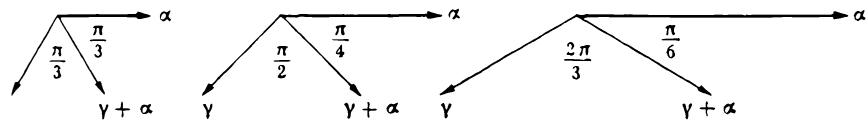
\includegraphics[keepaspectratio]{images/part001_d4d2d336.jpg}}

\begin{enumerate}
\def\labelenumi{\arabic{enumi})}
\setcounter{enumi}{2}
\tightlist
\item
  If the length of \(S\) is 2, then \(n(\gamma, \alpha) = -2\) , so
\end{enumerate}

\[
n (\alpha , \gamma) = - 1, (\alpha | \alpha) = \frac {1}{2} (\gamma | \gamma), (\alpha | \gamma) = - (\alpha | \alpha), \widehat {(\alpha , \gamma)} = \frac {3 \pi}{4}.
\]

\pandocbounded{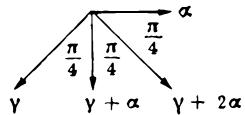
\includegraphics[keepaspectratio]{images/part001_f07fa75a.jpg}}

\begin{enumerate}
\def\labelenumi{\arabic{enumi})}
\setcounter{enumi}{3}
\tightlist
\item
  If the length of \(S\) is 3, then \(n(\gamma, \alpha) = -3\) , so
\end{enumerate}

\[
n (\alpha , \gamma) = - 1, (\alpha | \alpha) = \frac {1}{3} (\gamma | \gamma), (\alpha | \gamma) = - \frac {3}{2} (\alpha | \alpha), (\widehat {\alpha , \gamma}) = \frac {5 \pi}{6}.
\]

\pandocbounded{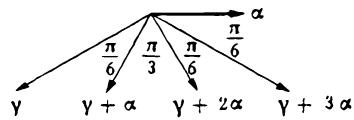
\includegraphics[keepaspectratio]{images/part001_9d247bec.jpg}}

We shall see (Plate X, Systems \(A_{2}, B_{2}, G_{2}\) ) that all these cases are actually realised.

PROPOSITION 10. Let \(\alpha, \beta\) be two non-proportional roots such that \(\beta + \alpha\) is a root. Let \(p, q\) be the integers in Prop. 9. Then

\[
\frac {(\beta + \alpha | \beta + \alpha)}{(\beta | \beta)} = \frac {q + 1}{p}.
\]

Let \(S\) be the \(\alpha\) -chain defined by \(\beta\) , \(\gamma\) its origin; its length \(l\) is \(\geqslant 1\) since \(\beta + \alpha\) is a root. The following cases are possible:

\begin{enumerate}
\def\labelenumi{\arabic{enumi})}
\item
  \(l = 1\) ; then \(\beta = \gamma, q = 0, p = 1, (\beta + \alpha | \beta + \alpha) = (\beta | \beta)\) .
\item
  \(l = 2\) , \(\beta = \gamma\) ; then \(q = 0\) , \(p = 2\) , \((\beta + \alpha|\beta + \alpha) = \frac{1}{2} (\beta|\beta)\) .
\item
  \(l = 2, \beta = \gamma + \alpha\) ; then \(q = 1, p = 1, (\beta + \alpha|\beta + \alpha) = 2(\beta|\beta)\) .
\item
  \(l = 3, \beta = \gamma\) ; then \(q = 0, p = 3, (\beta + \alpha | \beta + \alpha) = \frac{1}{3} (\beta | \beta)\) .
\item
  \(l = 3, \beta = \gamma + \alpha\) ; then \(q = 1, p = 2, (\beta + \alpha|\beta + \alpha) = (\beta|\beta)\) .
\item
  \(l = 3\) , \(\beta = \gamma + 2\alpha\) ; then \(q = 2, p = 1\) , \((\beta + \alpha|\beta + \alpha) = 3(\beta|\beta)\) .
\end{enumerate}

In each case, the formula to be proved is satisfied.

PROPOSITION 11. Assume that R is irreducible. Let \(\alpha\) and \(\beta\) be two roots such that \(\| \alpha \| = \| \beta \|\) . There exists \(g \in \mathrm{W}(\mathbb{R})\) such that \(g(\alpha) = \beta\) .

The transforms of \(\alpha\) by W(R) generate V (no. 2, Cor. of Prop. 5). Hence there exists \(g \in \mathrm{W}(\mathbb{R})\) such that \((g(\alpha)|\beta) \neq 0\) . We assume from now on that \((\alpha|\beta) \neq 0\) . By formula (9) of no. 1, \(n(\alpha, \beta) = n(\beta, \alpha)\) . Replacing \(\beta\) if necessary by \(s_{\beta}(\beta) = -\beta\) , we can assume that \(n(\alpha, \beta) > 0\) . Then, by the list at the beginning of no. 3, either \(\alpha = \beta\) (in which case the proposition is clear), or \(n(\alpha, \beta) = n(\beta, \alpha) = 1\) ; in that case

\[
s _ {\alpha} s _ {\beta} s _ {\alpha} (\beta) = s _ {\alpha} s _ {\beta} (\beta - \alpha) = s _ {\alpha} (- \beta - \alpha + \beta) = \alpha .
\]

\subsection{REDUCED ROOT SYSTEMS}

A root system is said to be reduced if every root of the system is indivisible (no. 3).

PROPOSITION 12. Assume that R is irreducible and reduced.

\begin{enumerate}
\def\labelenumi{(\roman{enumi})}
\item
  The ratio \(\frac{(\beta|\beta)}{(\alpha|\alpha)}\) for \(\alpha \in \mathbb{R}, \beta \in \mathbb{R}\) must take one of the values \(1, 2, \frac{1}{2}, 3, \frac{1}{3}\) .
\item
  The set of the \((\alpha |\alpha)\) for \(\alpha \in \mathrm{R}\) has at most two elements.
\end{enumerate}

Since R is irreducible, the transforms of a root by W(R) generate V (no. 2, Cor. of Prop. 5). Hence, for any roots \(\alpha, \beta\) , there exists a root \(\beta'\) such that \((\alpha|\beta') \neq 0\) and \((\beta'|\beta') = (\beta|\beta)\) . By formula (9) of no. 1 and the list of no. 3, \(\frac{(\beta'|\beta')}{(\alpha|\alpha)}\) takes one of the values \(1, 2, \frac{1}{2}, 3, \frac{1}{3}\) (recall that the system is assumed to be reduced). By multiplying \((x|y)\) by a suitable scalar, we can assume that \((\alpha|\alpha) = 1\) for certain roots and that the other possible values of \((\beta|\beta)\) for \(\beta \in \mathbb{R}\) are 2 and 3. The values 2 and 3 cannot both be attained, since in that case there would exist \(\beta \in \mathbb{R}, \gamma \in \mathbb{R}\) such that \(\frac{(\gamma|\gamma)}{(\beta|\beta)} = \frac{3}{2}\) , contrary to what we have seen above.

PROPOSITION 13. Assume that R is irreducible, non-reduced and of rank \(\geqslant 2\) .

\begin{enumerate}
\def\labelenumi{(\roman{enumi})}
\item
  The set \(\mathbf{R}_0\) of indivisible roots is a root system in V; this system is irreducible and reduced; and \(\mathrm{W}(\mathrm{R}_0) = \mathrm{W}(\mathrm{R})\) .
\item
  Let \(\mathbf{A}\) be the set of roots \(\alpha\) for which \((\alpha |\alpha)\) takes the smallest value \(\lambda\) . Then any two non-proportional elements of \(\mathbf{A}\) are orthogonal.
\item
  Let B be the set of \(\beta \in \mathbb{R}\) such that \((\beta |\beta) = 2\lambda\) . Then \(B \neq \emptyset\) , \(R_0 = A \cup B\) , \(R = A \cup B \cup 2A\) .
\end{enumerate}

If \(\alpha \in \mathbb{R} - \mathbb{R}_0\) , then \(\frac{1}{2}\alpha \in \mathbb{R}\) , but \(\frac{1}{2}\left(\frac{1}{2}\alpha\right) \notin \mathbb{R}\) (Prop. 8), so \(\frac{1}{2}\alpha \in \mathbb{R}_0\) . This proves that \(\mathbb{R}_0\) satisfies \((\mathrm{RS}_1)\) . It is clear that, for all \(\alpha \in \mathbb{R}\) , \(s_{\alpha, \alpha'}(\mathbb{R}_0) = \mathbb{R}_0\) , so \(\mathbb{R}_0\) satisfies \((\mathrm{RS}_{II})\) and \((\mathrm{RS}_{III})\) . Since \(\alpha \in \mathbb{R} - \mathbb{R}_0\) implies that \(\frac{1}{2}\alpha \in \mathbb{R}_0\) and since \(s_\alpha = s_{\alpha/2}\) , we have \(\mathrm{W}(\mathrm{R}) = \mathrm{W}(\mathrm{R}_0)\) . Thus \(\mathbb{R}_0\) is irreducible (Cor. of Prop. 5), and it is evidently reduced.

Since R is not reduced, there exists \(\alpha\in R_{0}\) such that \(2\alpha\in R\) . Since \(R_{0}\) is irreducible and \(\dim V\geqslant2\) , \(\alpha\) cannot be proportional or orthogonal to every root. Let \(\beta\in R_{0}\) be such that \(n(\beta,\alpha)\neq0\) and \(\beta\) is not proportional to \(\alpha\) . Changing \(\beta\) to \(-\beta\) if necessary, we can assume that \(n(\beta,\alpha)>0\) . Now \(\frac{1}{2}n(\beta,\alpha)=n(\beta,2\alpha)\in\mathbf{Z}\) , so \(n(\beta,\alpha)\in2\mathbf{Z}\) . From the list in no. 3, \(n(\beta,\alpha)=2\) , \((\beta|\beta)=2(\alpha|\alpha)\) . Since \(R_{0}\) is reduced, Prop. 12 shows that, for all \(\gamma\in R_{0}\) , either \((\gamma|\gamma)=(\alpha|\alpha)\) or \((\gamma|\gamma)=2(\alpha|\alpha)\) . Also, the above shows that, for all \(\gamma\in R-R_{0}\) , the vector \(\frac{1}{2}\gamma\) is an element of \(R_{0}\) such that \(\left(\frac{1}{2}\gamma|\frac{1}{2}\gamma\right)=(\alpha|\alpha)\) . Thus, \(\lambda=(\alpha|\alpha)\) , \(B\neq\varnothing\) , \(R_{0}=A\cup B\) , and \(R\subseteq A\cup B\cup2A\) ; on the other hand, if \(\gamma\in A\) , there exists \(g\in W(R)\) such that \(\gamma=g(\alpha)\) (Prop. 11), so \(2\gamma=g(2\alpha)\in R\) ; thus \(2A\subseteq R\) and \(R=A\cup B\cup2A\) . Finally, let \(\gamma,\gamma'\) be two non-proportional elements of A. Then

\[
n (2 \gamma , \gamma^ {\prime}) = 2 n (\gamma , \gamma^ {\prime}) = 4 n (\gamma , 2 \gamma^ {\prime}) \in 4 \mathbf {Z}, \text { and } | n (\gamma , \gamma^ {\prime}) | \leqslant 1
\]

since \(\gamma\) and \(\gamma'\) have the same length, so \(n(\gamma, \gamma') = 0\) and \((\gamma|\gamma') = 0\) .

PROPOSITION 14. Assume that R is irreducible and reduced, and that \((\alpha|\alpha)\) takes the values \(\lambda\) and \(2\lambda\) for \(\alpha\in R\) . Let A be the set of roots \(\alpha\) such that \((\alpha|\alpha)=\lambda\) . Assume that any two non-proportional elements of A are orthogonal. Then \(R_{1}=R\cup2A\) is an irreducible non-reduced root system and R is the set of indivisible roots of \(R_{1}\) .

It is clear that \(R_{1}\) satisfies \((RS_{I})\) and \((RS_{III})\) . We show that, if \(\alpha, \beta \in R_{1}\) , then \(\langle\alpha^{\sim}, \beta\rangle \in Z\) . This is clear if \(\alpha \in R\) . Since \((2\alpha)^{\sim} = \frac{1}{2}\alpha^{\sim}\) for \(\alpha \in A\) , it is also immediate if \(\alpha, \beta \in 2A\) . Finally, assume that \(\beta \in R\) and that \(\alpha = 2\gamma\) with \(\gamma \in A\) .

\begin{enumerate}
\def\labelenumi{\arabic{enumi})}
\item
  If \(\gamma = \pm \beta\) , then \(\langle \alpha^{\prime},\beta \rangle = \pm \frac{1}{2}\langle \gamma^{\prime},\gamma \rangle = \pm 1\) .
\item
  If \(\gamma\) is not proportional to \(\beta\) and if \(\beta \in A\) , the assumption on \(A\) implies that \(\langle \gamma^{\sim},\beta \rangle = 0\) , so \(\langle \alpha^{\sim},\beta \rangle = 0\) .
\item
  If \(\beta \in \mathbb{R} - \mathbb{A}\) , then \((\beta |\beta) = 2\lambda = 2(\gamma |\gamma)\) , so \(\langle \beta, \gamma^{\prime} \rangle\) is equal to 0, 2 or -2 by the list in no. 3. Thus \(\langle \beta, \alpha^{\prime} \rangle = \frac{1}{2}\langle \beta, \gamma^{\prime} \rangle \in \mathbf{Z}\) .
\end{enumerate}

Thus \(R_{1}\) is a root system in V, and the other assertions are clear.

\subsection{CHAMBERS AND BASES OF ROOT SYSTEMS}

For all \(\alpha \in \mathbb{R}\) , let \(L_{\alpha}\) be the hyperplane of \(V\) consisting of the points invariant under \(s_{\alpha}\) . The chambers in \(V\) determined by the set of the \(L_{\alpha}\) (Chap. V, § 1, no. 3) are called the chambers of \(R\) . The bijection \(V \to V^{*}\) defined by the scalar product \((x|y)\) takes \(\alpha\) to \(\frac{2\alpha^{-}}{(\alpha^{-}|\alpha^{-})}\) for \(\alpha \in R\) , hence \(L_{\alpha}\) to \(L_{\alpha^{-}}\) , and hence the chambers of \(R\) to those of \(R^{-}\) . If \(C\) is a chamber of \(R\) , the corresponding chamber of \(\mathbb{R}^{\sim}\) is denoted by \(\mathbb{C}^{\sim}\) . By Prop. 7 of no. 2, \(\mathbb{C}^{\sim}\) depends only on \(\mathbb{C}\) and not on the choice of \((x|y)\) .

THEOREM 2. (i) The group W(R) acts simply-transitively on the set of chambers.

\begin{enumerate}
\def\labelenumi{(\roman{enumi})}
\setcounter{enumi}{1}
\item
  Let \(\mathrm{C}\) be a chamber. Then \(\overline{\mathrm{C}}\) is a fundamental domain for \(\mathrm{W}(\mathrm{R})\) .
\item
  C is an open simplicial cone (Chap. V, § 1, no. 6).
\item
  Let \(L_{1}, L_{2}, \ldots, L_{l}\) be the walls of C. For all i, there exists a unique indivisible root \(\alpha_{i}\) such that \(L_{i} = L_{\alpha_{i}}\) and such that \(\alpha_{i}\) is on the same side of \(L_{i}\) as C.
\item
  The set B(C) = \(\{\alpha_{1},\ldots,\alpha_{l}\}\) is a basis of V.
\item
  C is the set of \(x \in V\) such that \(\langle \alpha_i, x \rangle > 0\) for all \(i\) (or, equivalently, the set of \(x \in V\) such that \((x|\alpha_i) > 0\) for all \(i\) ).
\item
  Let \(S\) be the set of the \(s_{\alpha_i}\) . The pair \((W(R), S)\) is a Coxeter system (Chap. IV, § 1, no. 3).
\end{enumerate}

Assertions (i) and (vii) follow from Chap. V, § 3, no. 2, Th. 1. Assertion (ii) follows from Chap. V, § 3, no. 3, Th. 2. Assertion (iv) is clear. The root \(\alpha_{i}\) is orthogonal to \(L_{i}\) , and \(\alpha_{i}^{-}\) is identified with \(2\alpha_{i}/(\alpha_{i}|\alpha_{i})\) . Since W(R) is essential (no. 1, Remark 3), assertions (iii), (v) and (vi) follow from Chap. V, § 3, no. 9, Prop. 7.

Remarks. 1) Assertion (vii) shows in particular that \(\mathrm{W}(\mathbb{R})\) is generated by the reflections \(s_{\alpha_i}\) .

\begin{enumerate}
\def\labelenumi{\arabic{enumi})}
\setcounter{enumi}{1}
\item
  If \(x, y \in \mathbb{C}\) , then \((x|y) > 0\) (Chap. V, § 3, no. 5, Lemma 6), in other words the angle \((\widehat{x,y})\) is acute.
\item
  Let \(m(\alpha, \beta)\) be the order of \(s_{\alpha} s_{\beta} (\alpha, \beta \in \mathrm{B}(\mathrm{C}))\) . The matrix \((m(\alpha, \beta))\) is identified with the Coxeter matrix (Chap. IV, § 1, no. 9) of (W, S). If \(\alpha \neq \beta\) , Prop. 3 of Chap. V, § 3, no. 4 shows that the angle \((\widehat{\alpha, \beta})\) is equal to \(\pi - \frac{\pi}{m(\alpha, \beta)}\) ; in particular, this angle is either obtuse or equal to \(\pi\) , and \((\alpha | \beta) \leqslant 0\) . By using the list in no. 3, it follows that \(m(\alpha, \beta)\) is equal to 2, 3, 4 or 6.
\end{enumerate}

DEFINITION 2. A subset B of R is called a basis of R if there exists a chamber C of R such that B = B(C). If C is a chamber, B(C) is called the basis of R defined by C.

Remarks. 4) Assertion (vi) of Th. 2 shows that the map C ↦ B(C) is a bijection from the set of chambers to the set of bases. Consequently, W(R) acts simply-transitively on the set of bases.

\begin{enumerate}
\def\labelenumi{\arabic{enumi})}
\setcounter{enumi}{4}
\tightlist
\item
  Let C be a chamber of R, and let B be the corresponding basis. If \(\alpha\in B\) , put \(\varphi(\alpha)=\alpha^{-}\) if \(2\alpha\notin R\) and \(\varphi(\alpha)=\frac{1}{2}\alpha^{-}\) if \(2\alpha\in R\) . Then \(\varphi(B)\) is the basis of \(R^{-}\) defined by \(C^{-}\) ; this follows from the fact that the walls of \(C^{-}\) are the \(L_{\alpha^{-}}\) , for \(\alpha\in B\) .
\end{enumerate}

DEFINITION 3. Let B be a basis of R. The Cartan matrix of R (relative to B) is the matrix \((n(\alpha,\beta))_{\alpha,\beta\in\mathbb{B}}\) .

For all \(\alpha \in \mathrm{B}\) , \(n(\alpha, \alpha) = 2\) . For \(\alpha, \beta \in \mathrm{B}\) ,

\[
n (\alpha , \beta) = 2 \frac {(\alpha | \beta)}{(\beta | \beta)} = - 2 \frac {\| \alpha \|}{\| \beta \|} \cos \frac {\pi}{m (\alpha , \beta)},\tag{11}
\]

where \(m(\alpha, \beta)\) denotes as above the order of \(s_{\alpha}s_{\beta}\) . If \(\alpha \neq \beta\) , \(n(\alpha, \beta) = 0\) , -1, -2 or -3 (cf.~no. 3).

Remarks. 6) The Cartan matrix \((n(\alpha,\beta))\) should not be confused with the Coxeter matrix \((m(\alpha,\beta))\) . Note in particular that the Cartan matrix is not necessarily symmetric.

\begin{enumerate}
\def\labelenumi{\arabic{enumi})}
\setcounter{enumi}{6}
\tightlist
\item
  Canonical indexing. If B and \(\mathbf{B}'\) are two bases of R, there exists a unique element \(w \in \mathbf{W}\) such that \(w(\mathbf{B}) = \mathbf{B}'\) . We have
\end{enumerate}

\[
n (w (\alpha), w (\beta)) = n (\alpha , \beta) \text { and } m (w (\alpha), w (\beta)) = m (\alpha , \beta)
\]

for \(\alpha, \beta \in \mathbf{B}\) . Consequently, the Cartan and Coxeter matrices associated to B can be obtained from those associated to \(\mathbf{B}'\) by composition with the bijection

\[
\alpha \mapsto w (\alpha)
\]

from B to B'.

The Cartan and Coxeter matrices can actually be defined canonically in the following way. Let X be the set of pairs \((B, \alpha)\) , where B is a basis of R and \(\alpha \in B\) . The group W acts in an obvious way on X and each orbit of W on X meets each of the sets \(\{B\} \times B\) in exactly one point. If I is the set of these orbits, each basis B admits a canonical indexing \((\alpha_{i})_{i \in I}\) . Moreover, there exists a unique matrix \(N = (n_{ij})\) (resp. \(M = (m_{ij})\) ), of type \(I \times I\) , such that for any basis B, the Cartan (resp. Coxeter) matrix associated to B can be obtained from N (resp. M) by composing with the canonical indexing of B; it is called the canonical Cartan matrix (resp. Coxeter matrix) of R.

PROPOSITION 15. Let B be a basis of R and \(\alpha\) an indivisible root. There exist \(\beta \in B\) and \(w \in W(R)\) such that \(\alpha = w(\beta)\) .

Let C be the chamber such that \(\mathrm{B} = \mathrm{B}(\mathrm{C})\) . The hyperplane \(L_{\alpha}\) is a wall of a chamber \(C'\) of R, and there exists an element of \(\mathrm{W}(\mathrm{R})\) that transforms \(C'\) to C. We are therefore reduced to the case where \(L_{\alpha}\) is a wall of C. Then \(\alpha\) is proportional to an element \(\beta\) of R. Since \(\alpha\) and \(\beta\) are indivisible, \(\alpha = \pm\beta\) . If \(\alpha = -\beta\) , then \(\alpha = s_{\beta}(\beta)\) , hence the proposition.

COROLLARY. Let \(R_{1}\) and \(R_{2}\) be two reduced root systems in vector spaces \(V_{1}\) and \(V_{2}\) , and let \(B_{1}\) and \(B_{2}\) be bases of \(R_{1}\) and \(R_{2}\) . Let \(f: B_{1} \to B_{2}\) be a bijection that transforms the Cartan matrix of \(R_{1}\) to that of \(R_{2}\) . Then there

exists an isomorphism \(\mathrm{F}: \mathrm{V}_1 \to \mathrm{V}_2\) that transforms \(\mathbb{R}_1\) to \(\mathbb{R}_2\) and \(\alpha\) to \(f(\alpha)\) for all \(\alpha \in \mathbb{B}_1\) .

Let F be the isomorphism from \(V_{1}\) to \(V_{2}\) that takes \(\alpha\) to \(f(\alpha)\) for all \(\alpha \in B_{1}\) . Then F transforms \(s_{\alpha}\) to \(s_{f(\alpha)}\) , hence \(W(R_{1})\) to \(W(R_{2})\) (Th. 2), and hence \(R_{1}\) to \(R_{2}\) (Prop. 15).

PROPOSITION 16. Let B be a basis of R, and G the subgroup of A(R) consisting of the elements leaving B stable. Then W(R) is a normal subgroup of A(R) and A(R) is the semi-direct product of G and W(R).

If \(\alpha\in R\) and \(t\in\mathrm{A}(\mathrm{R})\) , then \(ts_{\alpha}t^{-1}=s_{t(\alpha)}\) ; since \(\mathrm{W}(\mathrm{R})\) is generated by the \(s_{\alpha}\) , we see that \(\mathrm{W}(\mathrm{R})\) is a normal subgroup of \(\mathrm{A}(\mathrm{R})\) . By transport of structure, \(\mathrm{A}(\mathrm{R})\) transforms a basis of R to a basis of R. Since \(\mathrm{W}(\mathrm{R})\) acts simply-transitively on the set of bases, every element of \(\mathrm{A}(\mathrm{R})\) can be written uniquely in the form \(g_{1}g_{2}\) , where \(g_{1}\in\mathrm{W}(\mathrm{R})\) and \(g_{2}\in G\) .

Remarks. 8) Let \(\mathbb{R}_1, \ldots, \mathbb{R}_p\) be root systems in vector spaces \(\mathbb{V}_1, \ldots, \mathbb{V}_p\) , \(\mathbb{R}\) the direct sum of the \(\mathbb{R}_i\) in \(\mathbb{V} = \prod_i \mathbb{V}_i\) , \(\mathbb{C}_i\) a chamber of \(\mathbb{R}_i\) , and \(\mathbb{B}_i = \mathbb{B}(\mathbb{C}_i)\) . It is immediate that \(\mathbb{C} = \prod_i \mathbb{C}_i\) is a chamber of \(\mathbb{R}\) and that \(\mathbb{B}(\mathbb{C}) = \bigcup_i \mathbb{B}_i\) . It follows from Th. 2 that all the chambers and bases of \(\mathbb{R}\) are obtained in this way.

\subsection{POSITIVE ROOTS}

Let C be a chamber of R, and let \(\mathrm{B}(\mathrm{C})=\{\alpha_{1},\ldots,\alpha_{l}\}\) be the corresponding basis of R. The order relation on V (resp. \(V^{*}\) ) defined by C is the order relation compatible with the vector space structure of V (resp. \(V^{*}\) ) for which the elements \(\geqslant0\) are the linear combinations of the \(\alpha_{i}\) (resp. the \(\alpha_{i}^{-}\) ) with coefficients \(\geqslant0\) . An element that is positive for one of these relations is said to be positive for C, or positive for the basis \(\mathrm{B}(\mathrm{C})\) . These order relations are also defined by \(C^{-}\) , as one sees by identifying V with \(V^{*}\) by using a scalar product invariant under \(\mathrm{W}(\mathrm{R})\) . In view of Th. 2, no. 5, an element of \(V^{*}\) is \(\geqslant0\) if and only if its values on C are \(\geqslant0\) . An element x of V is \(\geqslant0\) if and only if its values on \(C^{-}\) are \(\geqslant0\) , or, equivalently, if \((x|y)\geqslant0\) for all \(y\in C\) .

The elements of \(\overline{C}\) are \(\geqslant 0\) for \(C\) by Lemma 6 of Chap. V, § 3, no. 5. But the set of elements \(\geqslant 0\) for \(C\) is in general distinct from \(\overline{C}\) (cf.~Plate X, Systems \(A_2\) , \(B_2\) , \(G_2\) ).

THEOREM 3. Every root is a linear combination with integer coefficients of the same sign of elements of B(C). In particular, every root is either positive or negative for C.

If \(\alpha \in \mathbb{R}\) , the kernel \(L_{\alpha}\) of \(\alpha\) does not meet \(C^{\cdot}\) , so \(\alpha\) is either \(>0\) on the whole of \(C^{\cdot}\) or \(< 0\) on the whole of \(C^{\cdot}\) , hence the second assertion. It remains to show that \(\alpha\) is contained in the subgroup \(P\) of \(V\) generated by \(B(C)\) ; we can assume that \(\alpha\) is indivisible. Now the group P is clearly stable under the \(s_{\gamma}\) , for \(\gamma \in \mathrm{B}(\mathrm{C})\) , hence also under \(\mathrm{W}(\mathrm{R})\) by Th. 2. Since \(\alpha\) is of the form \(w(\beta)\) , with \(w \in \mathrm{W}(\mathrm{R})\) and \(\beta \in \mathrm{B}(\mathrm{C})\) (cf.~Prop. 15), we have \(\alpha \in P\) . Q.E.D.

Denote by \(R_{+}(C)\) the set of roots that are positive for C. Thus,

\[
R = R _ {+} (C) \cup (- R _ {+} (C))
\]

is a partition of \(R\) .

COROLLARY. Let \(\gamma\) be a linear combination of roots with integer coefficients, and \(\alpha\) an indivisible root. If \(\gamma\) is proportional to \(\alpha\) , then \(\gamma \in Z\alpha\) .

By Prop. 15 of no. 5, C can be chosen so that \(\alpha \in B(C)\) . By Th. 3,

\[
\gamma = \sum_ {\beta \in B (C)} n _ {\beta} \beta \text {with} n _ {\beta} \in \mathbf {Z}.
\]

Thus, if \(\gamma\) is proportional to \(\alpha\) , then \(\gamma = n_{\alpha}\alpha\) , which proves the corollary.

Now let S be the set of reflections \(s_{\alpha}\) for \(\alpha \in \mathrm{B}(\mathrm{C})\) and let T be the union of the conjugates of S under W. For \(\alpha \in \mathrm{B}(\mathrm{C})\) and \(w \in W\) , the element \(t = ws_{\alpha}w^{-1}\) of T is the orthogonal reflection \(s_{\beta}\) associated to the root \(\beta = w(\alpha)\) ; conversely, for any indivisible root \(\beta\) , there exists an element \(w \in W\) such that \(\alpha = w^{-1}(\beta) \in \mathrm{B}(\mathrm{C})\) (Prop. 15) and \(s_{\beta} = ws_{\alpha}w^{-1} \in T\) . It follows that a bijection \(\psi\) from the set of indivisible roots to \(\{\pm1\} \times T\) is obtained by associating to an indivisible root \(\beta\) the pair \((\varepsilon, s_{\beta})\) , where \(\varepsilon = +1\) if \(\beta\) is positive and \(\varepsilon = -1\) if \(\beta\) is negative.

On the other hand, (W, S) is a Coxeter system (Th. 2) and the results of Chap. IV, § 1, no. 4 can be applied. We have seen that, if w is an element of W of length (with respect to S) equal to q, there exists a subset \(T_{w}\) of T, with q elements, such that, if \(w = s_{1} \ldots s_{q}\) with \(s_{i} \in S\) and if

\[
t _ {i} = s _ {1} \dots s _ {i - 1} s _ {i} s _ {i - 1} \dots s _ {1}
\]

(for \(1 \leqslant i \leqslant q\) ), then \(\mathrm{T}_w = \{t_1, \ldots, t_q\}\) . Recall that we have also defined in no. 4 of § 1 a number \(\eta(w, t)\) (for \(w \in \mathrm{W}\) and \(t \in \mathrm{T}\) ) equal to \(+1\) if \(t \notin \mathrm{T}_w\) and to \(-1\) if \(t \in \mathrm{T}_w\) . Finally, recall that, if we define a map \(\mathrm{U}_w\) from the set \(\{\pm 1\} \times \mathrm{T}\) to itself by the formula

\[
\mathbf {U} _ {w} (\varepsilon , t) = (\varepsilon \eta (w ^ {- 1}, t), w t w ^ {- 1}),
\]

the map \(w \mapsto \mathrm{U}_w\) is a homomorphism from \(W\) to the group of permutations of the set \(\{\pm 1\} \times T\) (Chap. IV, §1, no. 4, Lemma 1).

PROPOSITION 17. Assume that R is reduced and let \(w \in W\) and \(\alpha \in R\) .

\begin{enumerate}
\def\labelenumi{(\roman{enumi})}
\item
  We have \(\psi(w(\alpha)) = U_w(\psi(\alpha)).\)
\item
  Assume that \(\alpha\) is positive. The root \(w(\alpha)\) is negative if and only if
\end{enumerate}

\[
\eta (w ^ {- 1}, s _ {\alpha}) = - 1,
\]

in other words if \(s_{\alpha} \in \mathrm{T}_{w^{-1}}\) .

\begin{enumerate}
\def\labelenumi{(\roman{enumi})}
\setcounter{enumi}{2}
\tightlist
\item
  We have \(\eta(w,s_{\alpha})=-1\) if and only if the chambers C and \(w(C)\) are on opposite sides of the hyperplane \(L_{\alpha}\) . In other words, the set \(T_{w}\) consists of the reflections with respect to the walls separating C and \(w(C)\) .
\end{enumerate}

Let \(\beta \in \mathrm{B}(\mathrm{C})\) and put \(s = s_{\beta}\) . Clearly \(\mathrm{T}_s = \{s\}\) and consequently

\[
\mathrm{U} _ {s} (\varepsilon , t) = \left\{ \begin{array}{l l} (\varepsilon , s t s ^ {- 1}) & \text { if } t \neq s \\ (- \varepsilon , s) & \text { if } t = s. \end{array} \right.\tag{12}
\]

On the other hand, let \(\rho = \sum_{\gamma \in B(C)} n_{\gamma}(\rho) \gamma\) be a positive root. Put

\[
s (\rho) = \sum_ {\gamma \in B (C)} n _ {\gamma} (s (\rho)) \gamma .
\]

If \(\rho \neq \beta\) , there exists an element \(\gamma \in \mathrm{B}(\mathbf{C})\) with \(\gamma \neq \beta\) , such that \(n_{\gamma}(\rho) > 0\) , and we have \(n_{\gamma}(s(\rho)) = n_{\gamma}(\rho) > 0\) (no. 1, formula (5)). Hence \(s(\rho)\) is positive. We deduce immediately that

\[
\psi (s (\varepsilon . \rho)) = \left\{ \begin{array}{l l} (\varepsilon , s s _ {\rho} s ^ {- 1}) & \text {if} \rho \neq \beta \\ (- \varepsilon , s) & \text {if} \rho = \beta . \end{array} \right.\tag{13}
\]

Comparison of (12) and (13) now shows that \(\mathrm{U}_{s}(\psi(\gamma)) = \psi(s(\gamma))\) for all roots \(\gamma\) and all \(s \in S\) . Since S generates W, (i) follows.

On the other hand, saying that \(w(\alpha)\) is negative is equivalent to saying that

\[
\psi (w (\alpha)) = (- 1, w s _ {\alpha} w ^ {- 1}),
\]

or, by (i), that \(\mathrm{U}_w(\psi (\alpha)) = (-1, ws_{\alpha}w^{-1})\) . If in addition \(\alpha\) is positive, then \(\psi (\alpha) = (+1,s_{\alpha})\) and \(\mathrm{U}_w(\psi (\alpha)) = (\eta (w^{-1},s_{\alpha}),ws_{\alpha}w^{-1})\) , hence (ii).

Finally, by (ii), \(\eta(w,s_{\alpha})=-1\) if and only if one of the roots \(\alpha\) and \(w^{-1}(\alpha)\) is positive and the other negative. This is equivalent to saying that \((\alpha|x).(w^{-1}(\alpha)|x)=(\alpha|x).( \alpha|w(x))<0\) for all \(x\in C\) , hence the first assertion in (iii). The second assertion in (iii) follows immediately.

COROLLARY 1. Let \(\beta \in \mathrm{B}(\mathbb{C})\) . The reflection \(s_{\beta}\) permutes the positive roots not proportional to \(\beta\) .

We reduce immediately to the case in which R is reduced. In that case, our assertion follows from (ii) and the fact that \(T_{s_{\beta}} = s_{\beta}\) .

COROLLARY 2. Assume that R is reduced. Let \(w \in W\) , let \(q\) be the length of \(w\) with respect to S (Chap. IV, § 1, no. 1), and let \(w = s_1 \ldots s_q\) be a reduced decomposition of \(w\) . Let \(\alpha_1, \ldots, \alpha_q\) be the elements of B(C) corresponding to \(s_1, \ldots, s_q\) . Put

\[
\theta_ {i} = s _ {q} s _ {q - 1} \dots s _ {i + 1} (\alpha_ {i}), \quad i = 1, \dots , q.
\]

The roots \(\theta_{i}\) are \(>0\) , pairwise distinct, \(w(\theta_{i}) < 0\) , and every root \(\alpha > 0\) such that \(w(\alpha) < 0\) is equal to one of the \(\theta_{i}\) .

Let \(X\) be the set of \(\alpha > 0\) such that \(w(\alpha) < 0\) . By (ii),

\[
\operatorname{Card} (X) = \operatorname{Card} \left(T _ {w ^ {- 1}}\right) = l \left(w ^ {- 1}\right) = l (w) = q.
\]

On the other hand, if \(\alpha \in X\) it is clear that there exists \(i \in [1, q]\) such that

\[
s _ {i + 1} \ldots s _ {q} (\alpha) > 0 \quad \text {and} \quad s _ {i} s _ {i + 1} \ldots s _ {q} (\alpha) <   0.
\]

By Cor. 1, this implies that \(s_i s_{i+1} \ldots s_q(\alpha) = \alpha_i\) and hence that \(\alpha = \theta_i\) . The set X is thus contained in the set of \(\theta_i\) . Since \(\text{Card}(X) = q\) , this is possible only if X is equal to the set of \(\theta_i\) and these are pairwise distinct. Hence the corollary.

COROLLARY 3. Assume that R is reduced. There exists a unique longest element \(w_0\) in W. Its length is equal to the number of positive roots and \(w_0\) transforms the chamber C to -C. We have \(w_0^2 = 1\) and \(l(ww_0) = l(w_0) - l(w)\) for all \(w \in W\) .

It is clear that -C is a chamber. Hence there exists an element \(w_{0}\) of W that transforms C to -C. Then \(w_{0}(\alpha) < 0\) for all positive roots \(\alpha\) and the first two assertions of Cor. 3 are immediate consequences of Cor. 2. We have \(w_{0}^{2}(C) = C\) , so \(w_{0}^{2} = 1\) . Finally, if \(w \in W\) , the length \(l(w)\) (resp. \(l(ww_{0})\) ) is equal, by Prop. 17 (iii), to the number of walls separating C and \(w(C)\) (resp. \(ww_{0}(C) = -w(C)\) ). Since \(w(C)\) and \(-w(C)\) are on opposite sides of every wall, the sum \(l(w) + l(w_{0})\) is equal to the total number of walls, that is to \(l(w_{0})\) .

PROPOSITION 18. Let \(x \in V\) . The following three properties are equivalent:

\begin{enumerate}
\def\labelenumi{(\roman{enumi})}
\item
  \(x \in \overline{C};\)
\item
  \(x \geqslant s_{\alpha}(x)\) for all \(\alpha \in \mathrm{B}(\mathrm{C})\) (with respect to the order relation defined by \(\mathrm{C}\) );
\item
  \(x \geqslant w(x)\) for all \(w \in W\) .
\end{enumerate}

Since \(s_{\alpha}(x) = x - \langle x, \alpha' \rangle \alpha\) and since \(\overline{\mathbf{C}}\) is the set of elements \(x \in V\) such that \(\langle x, \alpha' \rangle \geqslant 0\) for all \(\alpha \in \mathrm{B}(\mathbf{C})\) , the equivalence of (i) and (ii) is obvious. On the other hand, it is clear that (iii) \(\Longrightarrow\) (ii). We show that (i) \(\Longrightarrow\) (iii). Let \(x \in \overline{\mathbf{C}}\) , and let \(w \in W\) . We argue by induction on the length \(l(w)\) of \(w\) . The case \(l(w) = 0\) is trivial. If \(l(w) \geqslant 1\) , \(w\) can be written in the form \(w = w's_{\alpha}\) , with \(\alpha \in \mathrm{B}(\mathbf{C})\) and \(l(w') = l(w) - 1\) . Then

\[
x - w (x) = x - w ^ {\prime} (x) + w ^ {\prime} \left(x - s _ {\alpha} (x)\right).
\]

The induction hypothesis shows that \(x - w'(x)\) is positive. On the other hand,

\[
w ^ {\prime} (x - s _ {\alpha} (x)) = w \left(s _ {\alpha} (x) - x\right) = - \langle x, \alpha^ {*} \rangle w (\alpha).
\]

Now \(s_{\alpha} \in T_{w^{-1}}\) , and Prop. 17 (ii) shows that \(w(\alpha) < 0\) . Hence the result.

COROLLARY. An element \(x \in \mathbf{C}\) if and only if \(x > w(x)\) for all \(w \in \mathbf{W}\) such that \(w \neq 1\) .

PROPOSITION 19. Let \((\beta_{i})_{1\leqslant i\leqslant n}\) be a sequence of positive roots for the chamber C such that \(\beta_{1}+\beta_{2}+\cdots+\beta_{n}\) is a root. Then there exists a permutation \(\pi\in S_{n}\) such that, for all \(i\in\{1,2,\ldots,n\}\) , \(\beta_{\pi(1)}+\beta_{\pi(2)}+\cdots+\beta_{\pi(i)}\) is a root.

We argue by induction on n, the proposition being clear for \(n \leqslant 2\) . Put \(\beta = \beta_{1} + \cdots + \beta_{n}\) . Then \(\sum_{i=1}^{n} (\beta | \beta_{i}) = (\beta | \beta) > 0\) , so there exists an index k such that \((\beta | \beta_{k}) > 0\) . If \(\beta = \beta_{k}\) , then n = 1 since \(\beta_{i} > 0\) for all i. Otherwise \(\beta - \beta_{k}\) is a root (no. 3, Cor. of Th. 1); it then suffices to apply the induction hypothesis to \(\beta - \beta_{k} = \sum_{i \neq k} \beta_{i}\) .

COROLLARY 1. Let \(\alpha \in \mathrm{R}_{+}(\mathrm{C})\) . Then \(\alpha \in \mathrm{B}(\mathrm{C})\) if and only if \(\alpha\) is the sum of two positive roots.

If \(\alpha\) is the sum of two positive roots, Th. 3 shows that \(\alpha \in \mathrm{B}(\mathrm{C})\) . If \(\alpha \notin \mathrm{B}(\mathrm{C})\) , Th. 3 shows that \(\alpha = \sum_{k=1}^{n} \beta_k\) with \(\beta_k \in \mathrm{B}(\mathrm{C})\) for all \(k\) and \(n \geqslant 2\) . Permuting the \(\beta_k\) if necessary, we can assume that \(\sum_{k=1}^{n-1}\) is a root (Prop. 19), and hence that \(\alpha\) is the sum of the positive roots \(\sum_{k=1}^{n-1} \beta_k\) and \(\beta_n\) .

COROLLARY 2. Let \(\varphi\) be a map from \(R\) to a abelian group \(\Gamma\) having the following properties:

\begin{enumerate}
\def\labelenumi{\arabic{enumi})}
\item
  \(\varphi(-\alpha) = -\varphi(\alpha)\) for \(\alpha \in \mathbf{R}\) ;
\item
  if \(\alpha \in \mathrm{R}\) , \(\beta \in \mathrm{R}\) are such that \(\alpha + \beta \in \mathrm{R}\) , then \(\varphi(\alpha + \beta) = \varphi(\alpha) + \varphi(\beta)\) .
\end{enumerate}

Let \(\mathbf{Q}\) be the subgroup of \(\mathbf{V}\) generated by \(\mathbf{R}\) . Then \(\varphi\) extends to a homomorphism from \(\mathbf{Q}\) to \(\Gamma\) .

Let B be a basis of R. Let \(\psi\) be the unique homomorphism from Q to \(\Gamma\) that coincides with \(\varphi\) on B. It suffices to show that \(\psi(\alpha) = \varphi(\alpha)\) when \(\alpha\) is a positive root relative to B. We have \(\alpha = \beta_{1} + \cdots + \beta_{m}\) with \(\beta_{i} \in B\) for all i, and \(\beta_{1} + \cdots + \beta_{h} \in R\) for all h (Prop. 19). We show that \(\psi(\alpha) = \varphi(\alpha)\) by induction on m. This is clear if m = 1. The induction hypothesis gives

\[
\psi \left(\beta_ {1} + \dots + \beta_ {m - 1}\right) = \varphi \left(\beta_ {1} + \dots + \beta_ {m - 1}\right),
\]

and we have \(\psi (\beta_m) = \varphi (\beta_m)\) , hence \(\psi (\alpha) = \varphi (\alpha)\) , which proves the corollary.

For any root \(\alpha = \sum_{\beta \in \mathrm{B}(\mathbb{C})} n_{\beta} \beta\) in \(\mathbb{R}\) , denote by \(\Upsilon(\alpha)\) the set of \(\beta \in \mathrm{B}(\mathbb{C})\) such that \(n_{\beta} \neq 0\) . Moreover, observe that \(\mathrm{B}(\mathbb{C})\) can be identified with the set of vertices of the graph of the Coxeter system formed by \(\mathrm{W}(\mathbb{R})\) and the \(s_{\alpha_i}\) (cf.~Chap. IV, § 1, no. 9 and Chap. V, § 3, no. 2).

COROLLARY 3. a) Let \(\alpha \in \mathbb{R}\) . Then \(\mathrm{Y}(\alpha)\) is a connected subset of \(\mathrm{B}(\mathrm{C})\) (Chap. IV, Appendix).

\begin{enumerate}
\def\labelenumi{\alph{enumi})}
\setcounter{enumi}{1}
\tightlist
\item
  Let Y be a non-empty connected subset of B(C). Then \(\sum_{\beta\in Y}\beta\) belongs to R.
\end{enumerate}

To prove \(a\) ), we can assume that \(\alpha\) is positive. We argue by induction on \(\operatorname{Card}(\mathbf{Y}(\alpha))\) , the assertion being trivial if \(\operatorname{Card}(\mathbf{Y}(\alpha)) = 1\) . By Prop. 19, there exists \(\beta \in \mathrm{B}(\mathrm{C})\) such that \(\alpha - \beta \in \mathrm{R}\) . Let \(p\) be the largest integer \(\geqslant 0\) such that \(\gamma = \alpha - p\beta \in \mathrm{R}\) . Since \(\gamma - \beta \notin \mathrm{R}\) and \(\gamma + p\beta \in \mathrm{R}\) , \((\gamma|\beta) \neq 0\) (Prop. 9); thus \(\beta\) is linked to at least one element of \(\mathbf{Y}(\gamma)\) . But \(\mathbf{Y}(\alpha) = \mathbf{Y}(\gamma) \cup \{\beta\}\) , and \(\mathbf{Y}(\gamma)\) is connected by the induction hypothesis. Thus \(\mathbf{Y}(\alpha)\) is connected, which proves \(a\) ).

Now let Y be a non-empty connected subset of B(C); we show by induction on \(\operatorname{Card}(Y)\) that \(\sum_{\beta\in Y}\beta\) is a root. The case in which \(\operatorname{Card}(Y)\leqslant1\) is trivial. Assume that \(\operatorname{Card}(Y)\geqslant2\) . Since X is a forest (Chap. V, § 4, no. 8, Prop. 8), Y is a tree and has a terminal vertex \(\beta\) (Chap. IV, Appendix). The set \(Y-\{\beta\}\) is connected, and one of its element is linked to \(\beta\) . By the induction hypothesis, \(\alpha=\sum_{\gamma\in Y-\{\beta\}}\gamma\in R\) , and since \((\alpha|\beta)<0\) , it follows that \(\alpha+\beta\in R\) (Th. 1). Q.E.D.

\subsection{CLOSED SETS OF ROOTS}

DEFINITION 4. Let P be a subset of R.

\begin{enumerate}
\def\labelenumi{(\roman{enumi})}
\item
  P is said to be closed if the conditions \(\alpha \in \mathrm{P},\beta \in \mathrm{P},\alpha +\beta \in \mathrm{R}\) imply \(\alpha +\beta \in \mathrm{P}\) .
\item
  P is said to be parabolic if P is closed and if \(\mathrm{P} \cup (-\mathrm{P}) = \mathrm{R}\) .
\item
  P is said to be symmetric if \(\mathrm{P} = -\mathrm{P}\) .
\end{enumerate}

Lemma 3. Let C be a chamber of R and P a closed subset of R containing \(\mathrm{R}_{+}(\mathrm{C})\) (in the notation of no. 6). Let \(\Sigma = \mathrm{B}(\mathrm{C}) \cap (-\mathrm{P})\) , and let Q be the set of roots that are linear combinations of elements of \(\Sigma\) with non-positive integer coefficient. Then, \(\mathrm{P} = \mathrm{R}_{+}(\mathrm{C}) \cup \mathrm{Q}\) .

It is enough to show that \(P \cap (-R_{+}(C)) = Q\) . Let \(-\alpha \in Q\) . Then \(\alpha\) is the sum of n elements of \(\Sigma\) . We show, by induction on n, that \(-\alpha \in P\) . This is clear if n = 1. If n \textgreater{} 1, then by Prop. 19 of no. 6 we can write \(\alpha = \beta + \gamma\) with \(\gamma \in \Sigma\) and \(\beta\) the sum of n - 1 elements of \(\Sigma\) . By the induction hypothesis, \(-\beta \in P\) ; since \(-\gamma \in P\) and since P is closed, \(-\alpha \in P\) . Thus, \(Q \subseteq P \cap (-R_{+}(C))\) . Conversely, let \(-\alpha \in P \cap (-R_{+}(C))\) . Then \(\alpha\) is the sum of p elements of B(C). We show, by induction on p, that \(-\alpha \in Q\) . This is clear if p = 1. If p \textgreater{} 1, then by Prop. 19, we can write \(\alpha = \beta + \gamma\) with \(\gamma \in B(C)\) and \(\beta\) a root that is the sum of p - 1 elements of B(C). Since \(-\gamma = \beta + (-\alpha)\) and since P is closed, \(-\gamma \in P\) , hence \(\gamma \in \Sigma\) . Moreover, \(-\beta = \gamma + (-\alpha) \text{ so } -\beta \in \mathbf{P} \text{ since P is closed. By the induction hypothesis, } -\beta \in \mathbf{Q}, \text{ so } -\alpha = -\beta - \gamma \in \mathbf{Q}\) . Thus, \(\mathrm{P} \cap (-\mathrm{R}_{+}(\mathrm{C})) \subseteq \mathrm{Q}\) .

PROPOSITION 20. Let P be a subset of R. The following conditions are equivalent:

\begin{enumerate}
\def\labelenumi{(\roman{enumi})}
\item
  P is parabolic;
\item
  P is closed and there exists a chamber C of R such that \(\mathrm{P} \supseteq \mathrm{R}_{+}(\mathrm{C})\) ;
\item
  there exist a chamber C of R and a subset \(\Sigma\) of B(C) such that P is the union of \(\mathrm{R}_{+}(\mathrm{C})\) and the set Q of roots that are linear combinations of elements of \(\Sigma\) with non-positive integer coefficients.
\item
  \(\Longrightarrow\) (iii): this follows from Lemma 3.
\item
  \(\Longrightarrow\) (i): we adopt the assumptions and notation of (iii). It is clear that \(\mathrm{P} \cup (-\mathrm{P}) = \mathrm{R}\) . We show that, if \(\alpha, \beta \in \mathrm{P}\) are such that \(\alpha + \beta \in \mathrm{R}\) , then \(\alpha + \beta \in \mathrm{P}\) . This is obvious if the root \(\alpha + \beta\) is positive. Assume that \(\alpha + \beta\) is negative. Then \(\alpha + \beta = \sum_{\gamma \in \mathrm{B}(\mathbb{C})} n_{\gamma} \gamma\) , with \(n_{\gamma} \leqslant 0\) . But the coefficient of every element \(\gamma\) of \(\mathrm{B}(\mathbb{C}) - \Sigma\) in \(\alpha\) or \(\beta\) is \(\geqslant 0\) ; hence \(n_{\gamma} = 0\) if \(\gamma \in \mathrm{B}(\mathbb{C}) - \Sigma\) , so \(\alpha + \beta \in \mathbb{Q} \subseteq \mathbb{P}\) .
\item
  \(\Longrightarrow\) (ii): assume that P is parabolic. Let C be a chamber such that \(\operatorname{Card}(P\cap R_{+}(C))\) is as large as possible. Let \(\alpha\in\operatorname{B}(C)\) and assume that \(\alpha\in P\) , so that \(-\alpha\in P\) . For all \(\beta\in P\cap R_{+}(C)\) , \(\beta\) is not proportional to \(\alpha\) (for the hypothesis \(\beta=2\alpha\) would imply that \(\alpha=2\alpha+(-\alpha)\in P\) since P is closed). Thus \(s_{\alpha}(\beta)\in\operatorname{R}_{+}(C)\) (no. 6, Cor. 1 of Prop. 17). If we put \(C'=s_{\alpha}(C)\) , then \(\beta=s_{\alpha}(s_{\alpha}(\beta))\in s_{\alpha}(\operatorname{R}_{+}(C))=\operatorname{R}_{+}(C)\) , so \(-\alpha\in P\cap R_{+}(C')\) and hence \(\operatorname{Card}(P\cap R_{+}(C'))>\operatorname{Card}(P\cap R_{+}(C))\) . This is absurd, since \(\alpha\in P\) . Thus \(B(C)\subseteq P\) , and consequently \(R_{+}(C)\subseteq P\) by Prop. 19 and the fact that P is closed.
\end{enumerate}

COROLLARY 1. Let P be a subset of R. The following conditions are equivalent:

\begin{enumerate}
\def\labelenumi{(\roman{enumi})}
\item
  there exists a chamber C such that \(\mathrm{P} = \mathrm{R}_{+}(\mathrm{C})\) ;
\item
  P is closed and \(\{P, -P\}\) is a partition of R.
\end{enumerate}

The chamber C such that \(\mathrm{P} = \mathrm{R}_{+}(\mathrm{C})\) is then unique.

If \(\mathrm{P} = \mathrm{R}_{+}(\mathrm{C})\) , \(\mathrm{C}^{-}\) is the set of \(x^{*} \in \mathrm{V}^{*}\) such that \(\langle x^{*}, x \rangle > 0\) for all \(x \in \mathrm{P}\) , hence the uniqueness of \(\mathbf{C}\) .

COROLLARY 2. Assume that V is equipped with the structure of an ordered vector space such that, for this structure, every root of R is either positive or negative. Let P be the set of positive roots for this structure. Then there exists a unique chamber C of R such that \(P = R_{+}(C)\) .

Indeed, P satisfies condition (ii) of Cor. 1.

This corollary applies in particular when the order being considered is total, the condition on R then being automatically satisfied. Recall that such an order can be obtained, for example, by choosing a basis \((e_{i})_{1\leqslant i\leqslant n}\) of V and taking the lexicographic order on V, so \(x=\sum_{i}\xi_{i}e_{i}\) is \(\geqslant0\) if all the \(\xi_{i}\) are 0, or if \(\xi_{i}>0\) for the smallest index i such that \(\xi_{i}\neq0\) .

COROLLARY 3. A subset B of R is a basis of R if and only if the following conditions are satisfied:

\begin{enumerate}
\def\labelenumi{(\roman{enumi})}
\item
  the elements of B are linearly independent;
\item
  every root of R is a linear combination of elements of B in which the coefficients are either all positive or all negative;
\item
  every root of B is indivisible.
\end{enumerate}

We already know that the conditions are necessary (no. 5, Th. 2, and no. 6, Th. 3). Assume that conditions (i), (ii), (iii) are satisfied. Let P be the set of roots that are linear combinations of elements of B with coefficients \(\geqslant0\) . Since P satisfies condition (ii) of Cor. 1, there exists a chamber C such that \(P = R_{+}(C)\) ; let \(B' = B(C)\) , and let X and \(X'\) be the convex cones generated by B and \(B'\) . Then

\[
\mathrm{B} \subseteq \mathrm{P} \subseteq \mathrm{X} \quad \text { and } \quad \mathrm{B} ^ {\prime} \subseteq \mathrm{P} \subseteq \mathrm{X} ^ {\prime},
\]

which shows that X and \(X'\) are both generated by P, and hence coincide. But the half-lines generated by the elements of B (resp. by \(B'\) ) are the extreme generators of X (resp. \(X'\) ); since such a half-line contains only one indivisible root, \(B = B'\) .

COROLLARY 4. Let B be a basis of R, B' a subset of B, V' the vector subspace of V generated by B', and R' = R ∩ V'. Then B' is a basis of the root system R'.

This follows immediately from Cor. 3 and the Cor. of Prop. 4.

We call R' the root system generated by B'.

COROLLARY 5. Let B be a basis of R, \(A_{1}, A_{2}, \ldots, A_{r}\) pairwise orthogonal subsets of B, and \(A = A_{1} \cup A_{2} \cup \cdots \cup A_{r}\) . Then every root \(\alpha\) that is a linear combination of elements of A is actually a linear combination of elements of one of the \(A_{i}\) . In particular, if R is irreducible, there is no partition of B into pairwise orthogonal subsets.

Let \(E_1, \ldots, E_r\) , \(E\) be the vector subspaces of \(V\) generated by \(A_1, \ldots, A_r\) , \(A\) , respectively. By Cor. 4, we can assume that \(E = V\) . Then, by Th. 2 (vii) of no. 5, the \(E_i\) are stable under \(W(R)\) , so \(R\) is the union of the \(R \cap E_i\) (no. 2, Prop. 5).

COROLLARY 6. We adopt the hypotheses and notation of Prop. 20. Let \(V_{1}\) be the vector subspace of V generated by \(\Sigma\) . Then \(P \cap (-P) = Q \cup (-Q) = V_{1} \cap R\) is a root system in \(V_{1}\) with basis \(\Sigma\) .

We have \(P \cap (-P) = (R_{+}(C) \cup Q) \cap ((-R_{+}(C)) \cup (-Q)) = Q \cup (-Q)\) . Th. 3 proves that \(Q \cup (-Q) = V_{1} \cap R\) . Finally, \(\Sigma\) is a basis of the root system \(V_{1} \cap R\) by Cor. 4.

PROPOSITION 21. Let C (resp. C') be a chamber of R, \(\Sigma\) (resp. \(\Sigma'\) ) a subset of B(C) (resp. B(C')), Q (resp. Q') the set of linear combinations of elements of \(\Sigma\) (resp. \(\Sigma'\) ) with negative integer coefficients, and P = Q ∪ R \(_{+}\) (C) (resp. P' = Q' ∪ R \(_{+}\) (C')). If there exists an element of the Weyl group transforming P to P', then there exists an element of the Weyl group transforming C to C' and \(\Sigma\) to \(\Sigma'\) .

We reduce immediately to the case \(P = P'\) . Let \(V_1\) be the vector subspace of \(V\) generated by \(P \cap (-P)\) . Then \(\Sigma\) and \(\Sigma'\) are bases of the root system \(R_1 = P \cap (-P)\) in \(V_1\) (Cor. 6 of Prop. 20). Hence there exists \(g_1 \in W(R_1)\) such that \(g_1(\Sigma) = \Sigma'\) . It is clear that \(g_1\) is induced by an element \(g\) of \(W(R)\) , that is a product of the symmetries \(s_\sigma\) with \(\sigma \in \Sigma\) . Let \(\gamma = \sum_{\beta \in B(C)} c_\beta \beta\) be an element of \(P - R_1\) . Then \(c_\beta > 0\) for at least one \(\beta \in B(C) - \Sigma\) . Moreover, if \(\sigma \in \Sigma\) , then \(s_\sigma(\gamma) - \gamma \in V_1\) , so \(s_\sigma(\gamma)\) has at least one coordinate \(> 0\) with respect to \(B(C)\) (no. 1, formula (5)), hence \(s_\sigma(\gamma) \in R_+(C)\) and finally \(s_\sigma(\gamma) \in P - R_1\) . It follows that \(P - R_1\) is stable under the \(s_\sigma, \sigma \in \Sigma\) , and hence under \(g\) , so \(g(P) = P\) . We are thus reduced to proving the proposition when \(P = P'\) and \(\Sigma = \Sigma'\) . In this case, \(Q = Q'\) , so \(R_+(C) = P - Q = P - Q' = R_+(C')\) , and hence \(C = C'\) (Cor. 1 of Prop. 20).

COROLLARY. Let \(\mathrm{P}, \mathrm{P}'\) be two parabolic subsets of \(\mathbb{R}\) transformed into each other by an element of the Weyl group. If there exists a chamber \(\mathbb{C}\) of \(\mathbb{R}\) such that \(\mathrm{R}_{+}(\mathbb{C}) \subseteq \mathrm{P}\) and \(\mathrm{R}_{+}(\mathbb{C}) \subseteq \mathrm{P}'\) , then \(\mathrm{P} = \mathrm{P}'\) .

This follows from Lemma 3 and Prop. 21 since the only element of W(R) transforming C to C is 1, cf.~no. 5, Th. 2.

PROPOSITION 22. Let P be a closed subset of R such that \(P \cap (-P) = \varnothing\) . Then there exists a chamber C of R such that \(P \subseteq R_{+}(C)\) .

\begin{enumerate}
\def\labelenumi{\arabic{enumi})}
\item
  In view of the Cor. of Th. 1, no. 3, the assumptions \(\alpha \in \mathrm{P}\) , \(\beta \in \mathrm{P}\) , \((\alpha |\beta) < 0\) imply that \(\alpha + \beta \in \mathrm{P}\) .
\item
  We show that no sum \(\alpha_{1} + \cdots + \alpha_{q}\) ( \(q \geqslant 1\) ) of elements of P is zero. We proceed by induction on q. The assertion being clear for q = 1, assume that \(q \geqslant 2\) . If \(\alpha_{1} + \cdots + \alpha_{q} = 0\) , then
\end{enumerate}

\[
\alpha_ {1} = \alpha_ {2} + \dots + \alpha_ {q},
\]

so \((-\alpha_{1}|\alpha_{2}+\cdots+\alpha_{q})>0\) , hence there exists \(j\in[2,q]\) such that \((\alpha_{1}|\alpha_{j})<0\) . By part 1) of the proof, \(\alpha_{1}+\alpha_{j}\in P\) , and the relation \((\alpha_{1}+\alpha_{j})+\sum_{i\neq1,j}\alpha_{i}=0\) contradicts the induction hypothesis.

\begin{enumerate}
\def\labelenumi{\arabic{enumi})}
\setcounter{enumi}{2}
\tightlist
\item
  We show that there exists a non-zero element \(\gamma\) in V such that \((\gamma|\alpha) \geqslant 0\) for all \(\alpha \in P\) . If not, the result of 1) would show that an infinite sequence \(\alpha_{1}, \alpha_{2}, \ldots\) of elements of P could be found such that
\end{enumerate}

\[
\beta_ {i} = \alpha_ {1} + \dots + \alpha_ {i} \in P
\]

for all \(i\) ; there would exist two distinct integers \(i, j\) such that \(\beta_{i} = \beta_{j}\) , which would contradict the result of 2).

\begin{enumerate}
\def\labelenumi{\arabic{enumi})}
\setcounter{enumi}{3}
\tightlist
\item
  To prove the proposition, it is enough (Cor. 2 of Prop. 20) to show that there exists a basis \((\alpha_{k})_{1\leqslant k\leqslant l}\) of \(V\) such that, for the lexicographic order defined by this basis, every element of \(P\) is \(>0\) . We proceed by induction on \(l = \dim V\) , and assume that the proposition is established for all dimensions \(< l\) . Let \(\gamma \in V\) be such that \(\gamma \neq 0\) and \((\gamma |\alpha)\geqslant 0\) for all \(\alpha \in P\) (cf.~3)). Let \(L\) be the hyperplane orthogonal to \(\gamma\) , and \(V'\) the subspace of \(L\) generated by \(R\cap L\) . Then \(R\cap L\) is a root system in \(V'\) and \(P\cap L\) is closed in \(R\cap L\) . By the induction hypothesis, there exists a basis \((\beta_{1},\ldots ,\beta_{l'})\) of \(V'\) such that the elements of \(P\cap L\) are \(>0\) for the lexicographic order defined by this basis. Then any basis of \(V\) whose first \(l' + 1\) elements are \(\gamma ,\beta_{1},\ldots ,\beta_{l'}\) and whose remaining elements are in \(L\) has the required property.
\end{enumerate}

PROPOSITION 23. Let P be a subset of R and \(V_{1}\) (resp. \(\Gamma\) ) the vector subspace (resp. the subgroup) of V generated by P. The following conditions are equivalent:

\begin{enumerate}
\def\labelenumi{(\roman{enumi})}
\item
  P is closed and symmetric;
\item
  P is closed, and P is a root system in \(V_{1}\) ;
\item
  \(\Gamma \cap \mathbb{R} = \mathbb{P}\) .
\end{enumerate}

Assume that these conditions are satisfied. For any \(\alpha \in \mathbb{P}\) , let \(\alpha_{1}^{-}\) be the restriction of \(\alpha^{-}\) to \(\mathrm{V}_{1}\) . Then the map \(\alpha \mapsto \alpha_{1}^{-}\) is the canonical bijection from the root system \(\mathbb{P}\) to \(\mathbb{P}^{-}\) .

\begin{enumerate}
\def\labelenumi{(\roman{enumi})}
\setcounter{enumi}{2}
\item
  \(\Longrightarrow\) (i): clear.
\item
  \(\Longrightarrow\) (ii): assume that P is closed and symmetric. First, P satisfies \((\mathrm{RS}_{\mathrm{I}})\) in \(V_{1}\) . We show that, if \(\alpha, \beta \in P\) , then \(s_{\alpha}(\beta) \in P\) . This is clear if \(\alpha\) and \(\beta\) are proportional. Otherwise, \(s_{\alpha}(\beta) = \beta - n(\beta, \alpha)\alpha\) and \(\beta - p\alpha \in R\) for all rational integers p between 0 and \(n(\beta, \alpha)\) (Prop. 9, no. 3), so
\end{enumerate}

\[
\beta - n (\beta , \alpha) \alpha \in P
\]

since P is closed and symmetric. Thus, \(s_{\alpha,\alpha_{1}}(P) = P\) , and P satisfies \((RS_{II})\) . It is clear that P satisfies \((RS_{III})\) . Thus, P satisfies (ii), and we have proved the last assertion of the proposition at the same time.

\begin{enumerate}
\def\labelenumi{(\roman{enumi})}
\setcounter{enumi}{1}
\tightlist
\item
  \(\Longrightarrow\) (iii): we show that, if condition (ii) is satisfied, then \(\Gamma\cap R=P\) . It is clear that \(P\subseteq\Gamma\cap R\) . Let \(\beta\in\Gamma\cap R\) . Since \(\beta\in\Gamma\) and \(P=-P\) , \(\beta=\alpha_{1}+\alpha_{2}+\cdots+\alpha_{k}\) with \(\alpha_{1},\ldots,\alpha_{k}\in P\) . We shall prove that \(\beta\in P\) . This is clear if k=1. We argue by induction on k. We have
\end{enumerate}

\[
0 <   (\beta | \beta) = \sum_ {i = 1} ^ {k} (\beta | \alpha_ {i}),
\]

so \((\beta |\alpha_{i}) > 0\) for some index \(i\) . If \(\beta = \alpha_{i}\) , then \(\beta \in \mathbb{P}\) . Otherwise, \(\beta - \alpha_{i} \in \mathbb{R}\) (Cor. of Th. 1, no. 3), so \(\beta - \alpha_{i} \in \mathbb{P}\) by the induction hypothesis, hence \(\beta \in \mathbb{P}\) since \(\mathbb{P}\) is closed.

The conditions of Prop. 23 can be realised with \(V_{1} = V\) and yet \(P \neq R\) . For example, this is the case when \(R\) is a system of type \(G_{2}\) and \(P\) a system of type \(A_{2}\) ; cf.~Plate X.

PROPOSITION 24. Let R' be the intersection of R with a vector subspace of V, so that R' is a root system in the vector subspace V' that it generates (cf.~Cor. of Prop. 4, no. 1). Let B' be a basis of R'.

\begin{enumerate}
\def\labelenumi{(\roman{enumi})}
\item
  There exists a basis of R containing \(\mathbf{B}'\) .
\item
  \(\mathbf{R}'\) is the set of elements of \(\mathbf{R}\) that are linear combinations of elements of \(\mathbf{B}'\) .
\end{enumerate}

Assertion (ii) is clear. We prove (i). Let \((\varepsilon_{1},\varepsilon_{2},\ldots,\varepsilon_{l})\) be a basis of V such that \(B' = (\varepsilon_{p+1},\varepsilon_{p+2},\ldots,\varepsilon_{l})\) . The lexicographic order on V corresponding to this basis defines a chamber C of R. It is clear that every element of \(B'\) is minimal in \(\mathrm{R}_{+}(\mathrm{C})\) . Thus \(\mathrm{B}' \subseteq \mathrm{B}(\mathrm{C})\) .

\subsection{HIGHEST ROOT}

PROPOSITION 25. Assume that R is irreducible. Let C be a chamber of R, and let B(C) = \{ \(\alpha_{1}, \ldots, \alpha_{l}\) \} be the corresponding basis.

\begin{enumerate}
\def\labelenumi{(\roman{enumi})}
\item
  There exists a root \(\tilde{\alpha} = \sum_{i=1}^{l} n_i \alpha_i\) such that, for every root \(\sum_{i=1}^{l} p_i \alpha_i\) , we have \(n_1 \geqslant p_1, n_2 \geqslant p_2, \ldots, n_l \geqslant p_l\) . In other words, R has a largest element for the ordering defined by C.
\item
  We have \(\tilde{\alpha} \in \overline{\mathrm{C}}\) .
\item
  We have \((\tilde{\alpha}|\tilde{\alpha})\geqslant (\alpha |\alpha)\) for every root \(\alpha\)
\item
  For every positive root \(\alpha'\) not proportional to \(\tilde{\alpha}\) , we have \(n(\alpha', \tilde{\alpha}) = 0\) or 1.
\end{enumerate}

\begin{enumerate}
\def\labelenumi{\arabic{enumi})}
\item
  Let \(\alpha = \sum_{i=1}^{l} n_i \alpha_i\) , \(\beta = \sum_{i=1}^{l} p_i \alpha_i\) be two maximal roots for the ordering defined by C. We shall prove that \(\alpha = \beta\) , which will establish (i).
\item
  If \((\alpha | \alpha_i) < 0\) for some index \(i\) , it follows that either \(\alpha + \alpha_i \in \mathbb{R}\) or \(\alpha = -\alpha_i\) (Cor. of Th. 1, no. 3), and both possibilities are absurd by the maximality of \(\alpha\) . Thus \((\alpha | \alpha_i) \geqslant 0\) for all \(i\) .
\item
  If \(\alpha < 0\) , then \(\alpha < -\alpha\) , which is absurd. Thus \(n_i \geqslant 0\) for all \(i\) . Let \(J\) be the set of \(i\) such that \(n_i > 0\) , and \(J'\) the complement of \(J\) in \(\{1, 2, \ldots, l\}\) . Then \(J \neq \varnothing\) . If \(J'\) were non-empty, there would exist an \(i \in J\) and an \(i' \in J'\) such that \((\alpha_i | \alpha_{i'}) < 0\) (Cor. 5 of Prop. 20, no. 7); we would then have
\end{enumerate}

\[
\left(\alpha \mid \alpha_ {i ^ {\prime}}\right) = \sum_ {i \in \mathbf {I}} n _ {i} \left(\alpha_ {i} \mid \alpha_ {i ^ {\prime}}\right) <   0
\]

since \((\alpha_{j}|\alpha_{k})\leqslant 0\) whenever \(j\) and \(k\) are distinct, which would contradict 2). Thus \(J' = \emptyset\) and \(n_i > 0\) for all \(i\) .

\begin{enumerate}
\def\labelenumi{\arabic{enumi})}
\setcounter{enumi}{3}
\tightlist
\item
  We have \((\beta \mid \alpha_i) \geqslant 0\) for all \(i\) by 2). We cannot have \((\beta \mid \alpha_i) = 0\) for all \(i\) since \(\beta \neq 0\) . We deduce from 3) that
\end{enumerate}

\[
(\beta \mid \alpha) = \sum_ {i} n _ {i} (\beta \mid \alpha_ {i}) > 0.
\]

If \(\gamma = \alpha - \beta \in \mathbb{R}\) , either \(\alpha > \beta\) or \(\beta > \alpha\) (Th. 3, no. 6), which contradicts the maximality of \(\alpha\) and \(\beta\) . Thus \(\alpha = \beta\) (Cor. of Th. 1, no. 3).

\begin{enumerate}
\def\labelenumi{\arabic{enumi})}
\setcounter{enumi}{4}
\tightlist
\item
  By 2), \(\tilde{\alpha} \in \overline{C}\) . We shall prove that \((\alpha'|\alpha') \leqslant (\tilde{\alpha}|\tilde{\alpha})\) for every \(\alpha' \in R\) . Since \(\overline{C}\) is a fundamental domain for \(W(R)\) , we can assume that \(\alpha' \in \overline{C}\) . We have \(\tilde{\alpha} - \alpha' \geqslant 0\) , so \((\tilde{\alpha} - \alpha' | x) \geqslant 0\) for all \(x \in \overline{C}\) . In particular \((\tilde{\alpha} - \alpha' |\tilde{\alpha}) \geqslant 0\) and \((\tilde{\alpha} - \alpha' |\alpha') \geqslant 0\) , hence \((\tilde{\alpha}|\tilde{\alpha}) \geqslant (\alpha'|\tilde{\alpha}) \geqslant (\alpha'|\alpha')\) . Thus \(n(\alpha',\tilde{\alpha})\) must be equal to 0, 1 or -1 if \(\alpha'\) is not proportional to \(\tilde{\alpha}\) . If \(\alpha' \geqslant 0\) , then \((\tilde{\alpha}|\alpha') \geqslant 0\) by 2), so \(n(\alpha',\tilde{\alpha}) \geqslant 0\) and \(n(\alpha',\tilde{\alpha})\) must be either 0 or 1. Q.E.D.
\end{enumerate}

Remark. The root

\[
\tilde {\alpha} = \sum_ {i} n _ {i} \alpha_ {i}
\]

in (i) is said to be the highest root of R (with respect to C). Note that, by (i), we have \(n_{i} \geqslant 1\) for all i.

\subsection{WEIGHTS, RADICAL WEIGHTS}

Let \(l = \dim V\) . Denote by \(Q(R)\) the subgroup of \(V\) generated by \(R\) ; the elements of \(Q(R)\) are called the radical weights of \(R\) . By Th. 3 of no. 6, \(Q(R)\) is a discrete subgroup of \(V\) of rank \(l\) , and every basis of \(R\) is a basis of \(Q(R)\) .

Similarly, the group \(\mathrm{Q}(\mathsf{R}^{\cdot})\) is a discrete subgroup of \(V^{*}\) of rank l.

PROPOSITION 26. The set of \(x \in V\) such that \(\langle x, y^* \rangle \in \mathbf{Z}\) for all \(y^* \in Q(R^*)\) (or, equivalently, for all \(y^* \in R^*)\) is a discrete subgroup \(G\) of \(V\) containing \(Q(R)\) . If \(B'\) is a basis of \(R^*\) , the basis of \(V\) dual to \(B'\) is a basis of \(G\) .

Let \(x \in V\) . The following three properties are equivalent:

\begin{enumerate}
\def\labelenumi{(\roman{enumi})}
\item
  \(\langle x, y^{*} \rangle \in \mathbf{Z}\) for all \(y^{*} \in \mathrm{Q}(\mathrm{R}^{\vee})\) ;
\item
  \(\langle x, y^{*} \rangle \in Z\) for all \(y^{*} \in B'\) ;
\item
  the coordinates of \(x\) with respect to the dual basis of \(\mathbf{B}'\) are in \(\mathbf{Z}\) .
\end{enumerate}

We deduce from this that the basis dual to \(B'\) is a basis of \(G\) . On the other hand, \((RS_{\mathrm{III}})\) proves that \(R \subseteq G\) , so \(Q(R) \subseteq G\) .

The group G of Prop. 26 is denoted by P(R), and its elements are called the weights of R. We can also consider the group P(R') of weights of R'.

By Algebra, Chap. VII, 2nd edn., § 4, no. 8,

\[
\mathrm{P} (\mathrm{R}) / \mathrm{Q} (\mathrm{R}), \quad \mathrm{P} (\mathrm{R} ^ {\cdot}) / \mathrm{Q} (\mathrm{R} ^ {\cdot})
\]

are finite groups in duality over \(\mathbf{Q} / \mathbf{Z}\) , and hence are isomorphic. The common order of these two groups is called the connection index of R (or of R \(^{\sim}\) ).

If R is a direct sum of root systems \(R_{i}\) , the group \(Q(R)\) (resp. \(P(R)\) ) is identified canonically with the direct sum of the \(Q(R_{i})\) (resp. \(P(R_{i})\) ).

PROPOSITION 27. Let \(\mathbb{R}_1\) be a subset of \(\mathbb{R}\) , \(\mathbb{Q}_1\) the subgroup of \(\mathbb{Q}(\mathbb{R})\) generated by \(\mathbb{R}_1\) , and \(\mathbb{W}_1\) the subgroup of \(\mathbb{W}(\mathbb{R})\) generated by the \(s_\alpha\) ( \(\alpha \in \mathbb{R}_1\) ). If \(p \in \mathrm{P}(\mathbb{R})\) and \(w \in \mathbb{W}_1\) , then \(p - w(p) \in \mathbb{Q}_1\) .

If \(w = s_{\alpha}\) with \(\alpha \in \mathbb{R}_1\) , then

\[
p - w (p) = \langle p, \alpha^ {\prime} \rangle \alpha \in \mathbf {Z} \alpha \subseteq \mathrm{Q} _ {1}.
\]

If \(w = s_{\alpha_1}s_{\alpha_2}\ldots s_{\alpha_r}\) , with \(\alpha_{1},\ldots ,\alpha_{r}\in \mathbb{R}_{1}\) , it is still true that \(p - w(p)\in \mathbf{Q}_1\) , as we see by induction on \(r\) .

The group A(R) leaves P(R) and Q(R) invariant, and hence acts on the quotient P(R)/Q(R). By Prop. 27, the group W(R) acts trivially on P(R)/Q(R). Passing to the quotient, we see that the quotient group A(R)/W(R) (cf.~Prop. 16, no. 5) acts canonically on P(R)/Q(R).

\subsection{FUNDAMENTAL WEIGHTS, DOMINANT WEIGHTS}

Assume that R is reduced. Let C be a chamber of R, and let B be the corresponding basis of R. Since R is reduced, \(B^{-} = \{\alpha^{-}\}_{\alpha \in B}\) is a basis of \(R^{-}\) . The dual basis \((\overline{\omega}_{\alpha})_{\alpha \in B}\) of \(B^{-}\) is thus a basis of the group of weights; its elements are called the fundamental weights (relative to B, or to C); if the elements of B are denoted by \((\alpha_{1}, \ldots, \alpha_{l})\) , the corresponding fundamental weights are denoted by \((\overline{\omega}_{1}, \ldots, \overline{\omega}_{l})\) .

Let \(x \in V\) . Then, \(x \in C\) if and only if \(\langle x, \alpha \rangle > 0\) for all \(\alpha \in B\) . It follows that \(C\) is the set of linear combinations of the \(\bar{\omega}_{\alpha}\) with coefficients \(\geqslant 0\) .

The entries \(n(\alpha, \beta) = \langle \alpha, \beta' \rangle\) of the Cartan matrix are, for fixed \(\alpha\) , the coordinates of \(\alpha\) with respect to the basis \((\overline{\omega}_{\beta})_{\beta \in B}\) :

\[
\alpha = \sum_ {\beta \in B} n (\alpha , \beta) \overline {{\omega}} _ {\beta}.\tag{14}
\]

The Cartan matrix is thus the transpose of the matrix of the canonical injection

\[
\mathrm{Q} (\mathrm{R}) \rightarrow \mathrm{P} (\mathrm{R})
\]

with respect to the bases B and \((\overline{\omega}_{\alpha})_{\alpha\in\mathsf{B}}\) of the Z-modules \(\mathrm{Q}(\mathrm{R})\) and \(\mathrm{P}(\mathrm{R})\) . A weight \(\overline{\omega}\) is said to be dominant if it belongs to \(\overline{C}\) , in other words if its coordinates with respect to \((\overline{\omega}_{\alpha})_{\alpha\in\mathsf{B}}\) are integers \(\geqslant0\) , or equivalently if \(g(\overline{\omega})\leqslant\overline{\omega}\) for all \(g\in\mathrm{W}(\mathrm{R})\) (no. 6, Prop. 18). Since \(\overline{C}\) is a fundamental domain for \(\mathrm{W(R)}\) (Th. 2), there exists, for any weight \(\overline{\omega}\) , a unique weight \(\overline{\omega}'\) such that \(\overline{\omega}'\) is a transform of \(\overline{\omega}\) by \(\mathrm{W(R)}\) .

We have

\[
\langle \overline {{{{\omega}}}} _ {\alpha}, \beta^ {\prime} \rangle = (\overline {{{{\omega}}}} _ {\alpha} | \frac {2 \beta}{(\beta | \beta)}) = \delta_ {\alpha \beta}
\]

for \(\alpha, \beta \in \mathbf{B}\) ( \(\delta_{\alpha\beta}\) denoting the Kronecker symbol), hence

\[
s _ {\beta} (\overline {{\omega}} _ {\alpha}) = \overline {{\omega}} _ {\alpha} - \delta_ {\alpha \beta} \beta \quad \text { and } \quad (\overline {{\omega}} _ {\alpha} | \beta) = \frac {1}{2} (\beta | \beta) \delta_ {\alpha \beta}.
\]

In other words, \(\overline{\omega}_{\alpha}\) is orthogonal to \(\beta\) for \(\beta \neq \alpha\) , and its orthogonal projection onto \(R\alpha\) is \(\frac{1}{2}\alpha\) . Since \(\overline{\omega}_{\alpha} \in \overline{C}\) , \((\overline{\omega}_{\alpha} | \overline{\omega}_{\beta}) \geqslant 0\) for \(\alpha, \beta \in B\) , i.e.~the angle \((\widehat{\overline{\omega}_{\alpha}, \overline{\omega}_{\beta}})\) is acute or a right angle. The dominant weights are the \(\overline{\omega} \in V\) such that \(2(\overline{\omega} | \alpha)/( \alpha | \alpha)\) is an integer \(\geqslant 0\) for all \(\alpha \in B\) .

PROPOSITION 28. Let B be a basis of R, B' a subset of B, V' the vector subspace of V generated by B', R' = R ∩ V' (which is a root system in V'), R' the inverse root system (which is identified with the canonical image of R' in R'), V1 the orthogonal complement of R' in V, and p the projection of V onto V' parallel to V1. Then, Q(R') = Q(R) ∩ V', P(R') = p(P(R)). The set of dominant weights of R' is the image under p of the set of dominant weights of R.

Indeed, \(\mathrm{Q}(\mathrm{R})\) is the subgroup of \(\mathrm{V}\) with basis \(\mathrm{B}\) , \(\mathrm{Q}(\mathrm{R}')\) is the subgroup of \(\mathrm{V}'\) with basis \(\mathrm{B}'\) (no. 7, Cor. 4 of Prop. 20) from which \(\mathrm{Q}(\mathrm{R}') = \mathrm{Q}(\mathrm{R}) \cap \mathrm{V}'\) is immediate. If \(\overline{\omega} \in \mathrm{P}(\mathrm{R})\) and \(\alpha \in \mathrm{R}'\) , \(\langle p(\overline{\omega}), \alpha' \rangle = \langle \overline{\omega}, \alpha' \rangle \in \mathbf{Z}\) , so \(p(\overline{\omega}) \in \mathrm{P}(\mathrm{R}')\) , and hence \(p(\mathrm{P}(\mathrm{R})) \subseteq \mathrm{P}(\mathrm{R}')\) . If \(\overline{\omega}' \in \mathrm{P}(\mathrm{R}')\) , \(\overline{\omega}'\) extends to a linear form \(\overline{\omega}\) on \(\mathrm{V}^*\) vanishing on \((\mathrm{B} - \mathrm{B}')'\) ; we have \(\langle \overline{\omega}, \alpha' \rangle \in \mathbf{Z}\) for all \(\alpha \in \mathrm{B}\) , so \(\overline{\omega} \in \mathrm{P}(\mathrm{R})\) , and \(\overline{\omega}' = p(\overline{\omega})\) ; hence \(\mathrm{P}(\mathrm{R}') \subseteq p(\mathrm{P}(\mathrm{R}))\) . Thus \(\mathrm{P}(\mathrm{R}') = p(\mathrm{P}(\mathrm{R}))\) , and the assertion about dominant weights is proved in the same way.

PROPOSITION 29. Let \(\rho\) be half the sum of the roots \(>0\) .

\begin{enumerate}
\def\labelenumi{(\roman{enumi})}
\item
  \(\rho = \sum_{\alpha \in B} \overline{\omega}_{\alpha}\) ; this is an element of C.
\item
  \(s_{\alpha}(\rho) = \rho -\alpha\) for all \(\alpha \in B\)
\item
  \((2\rho |\alpha) = (\alpha |\alpha)\) for all \(\alpha \in B\) .
\end{enumerate}

Since R is reduced, \(s_{\alpha}(R_{+}(C) - \{\alpha\}) = R_{+}(C) - \{\alpha\}\) and \(s_{\alpha}(\alpha) = -\alpha\) for \(\alpha \in B\) (no. 6, Cor. 1 of Prop. 17), so \(s_{\alpha}(2\rho) = 2\rho - 2\alpha\) . Since \(s_{\alpha}(\rho) = \rho - \langle \rho, \alpha^{-} \rangle\) , we see that

\[
\langle \rho , \alpha^ {\prime} \rangle = 1 = \left\langle \sum_ {\beta \in B} \bar {\omega} _ {\beta}, \alpha^ {\prime} \right\rangle .
\]

Hence, \(\rho = \sum_{\beta} \overline{\omega}_{\beta}\) , and consequently \(\rho \in C\) . Finally, (iii) is equivalent to \(\langle \rho, \alpha^{-} \rangle = 1\) .

COROLLARY. Let \(\sigma\) be half the sum of the elements \(>0\) of \(\mathbf{R}^{-}\) (for \(\mathbf{B}^{-}\) ). For all \(\alpha \in V\) , the sum of the coordinates of \(\alpha\) with respect to the basis \(\mathbf{B}\) is \(\langle \alpha, \sigma \rangle\) . If \(\alpha \in R\) , this sum is equal to \(\frac{1}{2} \sum_{\beta \in \mathbb{R}_{+}(C)} n(\alpha, \beta)\) .

Interchanging the roles of R and \(R^{-}\) above, we have \(\langle\alpha,\sigma\rangle=1\) for all \(\alpha\in B\) , hence the corollary.

\subsection{COXETER TRANSFORMATION}

Let C be a chamber of R, let \(\{\alpha_{1},\ldots,\alpha_{l}\}\) be the corresponding basis of R, and let \(c=s_{\alpha_{1}}\ldots s_{\alpha_{l}}\) . The element c of W is called the Coxeter transformation of W defined by C and the bijection \(i\mapsto\alpha_{i}\) (Chap. V, § 6, no. 1). Its order h is called the Coxeter number of W (or of R).

PROPOSITION 30. Assume that R is irreducible. Let m be an integer between 1 and h - 1 and prime to h. Then \(\exp\left(\frac{2i\pi m}{h}\right)\) is an eigenvalue of c of multiplicity 1.

In particular, \(m\) is an exponent of \(W\) , cf.~Chap. V, § 6, no. 2.

We first prove a lemma:

Lemma 4. For all \(w \in W\) , the characteristic polynomial of \(w\) has integer coefficients.

We know (no. 6, Th. 3) that \(\{\alpha_{1},\ldots,\alpha_{l}\}\) is a basis of the subgroup \(Q(R)\) of V generated by R. Since w leaves \(Q(R)\) stable, its matrix with respect to \(\{\alpha_{1},\ldots,\alpha_{l}\}\) has integer entries; hence its characteristic polynomial has integer coefficients.

Let P be the characteristic polynomial of c.~The above lemma shows that the coefficients of P are integers. By Chap. V, § 6, no. 2, Cor. 2 of Prop. 3, the primitive hth root of unity \(z = \exp\left(\frac{2i\pi}{h}\right)\) is a simple root of P. Every conjugate of z over Q is therefore also a simple root of P. But we know (Algebra, Chap. V) that the primitive hth roots of unity are conjugate over Q. They are thus all simple roots of P, which proves the proposition.

PROPOSITION 31. Assume that R is irreducible and reduced, and let \(\beta = n_{1}\alpha_{1} + \cdots + n_{l}\alpha_{l}\) be the highest root of R (cf.~no. 8). Then \(n_{1} + \cdots + n_{l} = h - 1\) .

Let \(R_{+}\) be the set of positive roots relative to C. Then (no. 10, Cor. of Prop. 29):

\[
\begin{array}{l} n _ {1} + \dots + n _ {l} = \frac {1}{2} \sum_ {\alpha \in \mathrm{R} _ {+}} n (\beta , \alpha) \\ = 1 + \frac {1}{2} \sum_ {\alpha \in \mathrm{R} _ {+}, \alpha \neq \beta} n (\beta , \alpha) = 1 + \sum_ {\alpha \in \mathrm{R} _ {+}, \alpha \neq \beta} \frac {(\alpha | \beta)}{(\alpha | \alpha)}. \end{array}
\]

By no. 8, Prop. 25 (iv), for all \(\alpha \in \mathbb{R}_+\) and \(\alpha \neq \beta\) , \(n(\alpha, \beta) = 0\) or 1, so \(n(\alpha, \beta)^2 = n(\alpha, \beta)\) , that is \(\frac{4(\alpha | \beta)^2}{(\beta | \beta)^2} = \frac{2(\alpha | \beta)}{(\beta | \beta)}\) . Hence:

\[
\begin{array}{l} n _ {1} + \dots + n _ {l} + 1 = 2 + 2 \sum_ {\alpha \in R _ {+}, \alpha \neq \beta} \frac {(\alpha | \beta) ^ {2}}{(\alpha | \alpha) (\beta | \beta)} \\ = 2 \sum_ {\alpha \in R _ {+}} \frac {(\alpha | \beta) ^ {2}}{(\alpha | \alpha) (\beta | \beta)} = (\beta | \beta) ^ {- 1} \sum_ {\alpha \in R} (\frac {\alpha}{\| \alpha \|} | \beta) ^ {2}. \end{array}
\]

By Chap. V, § 6, no. 2, Cor. of Th. 1,

\[
\sum_ {\alpha \in R} \left(\frac {\alpha}{\| \alpha \|} | \beta\right) ^ {2} = h (\beta | \beta)
\]

\[
\mathrm{so} n _ {1} + \dots + n _ {l} + 1 = h.
\]

PROPOSITION 32. Assume that R is irreducible, and that all roots have the same length. Let \(\alpha \in R\) . The number of elements of R not orthogonal to \(\alpha\) is 4h - 6.

Let \(R'\) be the set of roots not proportional to and not orthogonal to \(\alpha\) . By Chap. V, § 6, no. 2, Cor. of Th. 1,

\[
(\alpha | \alpha) ^ {2} + (\alpha | - \alpha) ^ {2} + \sum_ {\beta \in \mathrm{R} ^ {\prime}} (\alpha | \beta) ^ {2} = h (\alpha | \alpha) ^ {2},
\]

that is

\[
\sum_ {\beta \in \mathsf {R} ^ {\prime}} (\alpha \mid \beta) ^ {2} = (h - 2) (\alpha \mid \alpha) ^ {2}.
\]

If \(\beta \in \mathbf{R}'\) , then \((\alpha | \beta) = \pm \frac{1}{2} (\alpha | \alpha)\) by the list in no. 3. Hence

\[
\frac {1}{4} \operatorname{Card} R ^ {\prime} = h - 2, \quad \operatorname{Card} R ^ {\prime} = 4 h - 8,
\]

and the number of roots not orthogonal to \(\alpha\) is \(\operatorname{Card} R' + 2 = 4h - 6\) .

PROPOSITION 33. Assume that R is irreducible and reduced. Put \(s_{\alpha_i} = s_i\) , and let \(\Gamma\) be the subgroup of W generated by \(c = s_1 \ldots s_l\) .

\begin{enumerate}
\def\labelenumi{(\roman{enumi})}
\item
  Let \(\theta_{i} = s_{l}s_{l - 1}\dots s_{i + 1}(\alpha_{i})\) ( \(i = 1,\dots ,l\) ). Then, \(\theta_{i} > 0,c(\theta_{i}) < 0\) .
\item
  If \(\alpha\) is a root \(>0\) such that \(c(\alpha) < 0\) , then \(\alpha\) is equal to one of the \(\theta_{i}\) .
\item
  The family \((\theta_{i})_{1\leqslant i\leqslant l}\) is a basis of \(\mathrm{Q}(\mathrm{R})\)
\item
  Let \(\Omega_{i}\) be the orbit of \(\theta_{i}\) under \(\Gamma\) . The sets \(\Omega_{i}\) are pairwise disjoint, they are all the orbits of \(\Gamma\) on \(\mathbb{R}\) , and each has \(h\) elements.
\end{enumerate}

Observe first that \((s_1, \ldots, s_l)\) is a reduced decomposition of \(c\) (Chap. IV, § 1, no. 1) with respect to the set \(S\) of the \(s_i\) . Indeed, otherwise there would exist a subset \(X = S - \{j\}\) of \(l - 1\) elements of \(S\) such that \(c \in W_X\) , which would contradict Cor. 2 of Prop. 7 of Chap. IV, § 1, no. 8.

Applying Cor. 2 of Prop. 17 of no. 6 to \(c\) gives assertions (i) and (ii).

Let \(Q_{i}\) be the subgroup of \(Q(R)\) generated by the \(\alpha_{j}, j > i\) . It is immediate that \(Q_{i}\) is stable under the \(s_{j}, j > i\) , and that \(s_{j}(\alpha_{i}) = \alpha_{i} \mod Q_{i}\) for \(j > i\) . Hence:

\[
\theta_ {i} = s _ {l} \dots s _ {i + 1} (\alpha_ {i}) = \alpha_ {i} \bmod . Q _ {i}.
\]

In other words, there exist integers \(c_{ij}\) such that

\[
\theta_ {i} = \alpha_ {i} + \sum_ {j > i} c _ {i j} \alpha_ {j}.
\]

Part (iii) follows immediately.

Finally, let \(\alpha\) be a root. The element \(\sum_{k=0}^{h-1} c^k(\alpha)\) is invariant under \(c\) , and hence zero (Chap. V, § 6, no. 2). The \(c^k(\alpha)\) cannot therefore all have the same sign, and there exists a \(k\) such that \(c^k(\alpha) > 0\) and \(c^{k+1}(\alpha) < 0\) . By (ii), \(c^k(\alpha)\) is one of the \(\theta_i\) . Thus every orbit of \(\Gamma\) on R is one of the \(\Omega_i\) . Extend \((x|y)\) to a hermitian form on V \(\otimes\) C. Each orbit of \(\Gamma\) in R has at most \(h\) elements, and there are at most \(l\) distinct orbits, by the above remarks. Now (Chap. V, § 6, no. 2, Theorem 2, ii)), the cardinal of R is equal to \(hl\) , which immediately implies (iv).
